% !TEX program = lualatex
\documentclass[a4paper,11pt,oneside,numbers=noenddot,headings=normal,bibliography=totoc,listof=totoc]{scrreprt}
\usepackage[a4paper,left=25mm,right=23mm,top=23mm,bottom=24mm,headsep=7mm]{geometry}
\usepackage{fontspec}
\usepackage{amsmath,mathtools,bm}
\usepackage{unicode-math}
\setmainfont{LibertinusSerif}[Extension=.otf,UprightFont=*-Regular,ItalicFont=*-Italic,BoldFont=*-Bold,BoldItalicFont=*-BoldItalic]
\setsansfont{LibertinusSans}[Extension=.otf,UprightFont=*-Regular,ItalicFont=*-Italic,BoldFont=*-Bold]
\setmathfont{LibertinusMath-Regular.otf}
\usepackage{microtype,siunitx,graphicx,subcaption,adjustbox}
\usepackage{booktabs,tabularx,longtable,threeparttable}
\usepackage{xcolor,tcolorbox,tikz}
\usetikzlibrary{arrows.meta,positioning}
\usepackage{listings,csquotes}
\usepackage[backend=biber,style=numeric-comp,sorting=none,maxbibnames=6,minbibnames=3,giveninits=true]{biblatex}
\addbibresource{references.bib}
\usepackage{hyperref,bookmark,cleveref,glossaries-extra,scrlayer-scrpage}
\definecolor{Navy}{HTML}{173A5E}
\definecolor{Teal}{HTML}{2E6F73}
\definecolor{Ink}{HTML}{20242A}
\definecolor{CoolGrey}{HTML}{F3F5F7}
\definecolor{Audit}{HTML}{A95542}
\hypersetup{hypertexnames=false,colorlinks=true,linkcolor=Navy,citecolor=Teal,urlcolor=Navy,pdftitle={RobustCluster-Aβ: reproducible analysis of amyloid-β40 conformational descriptors},pdfauthor={Ali Erkan Ocaklı},pdfsubject={Curricular internship report, Data Analysis L-31, academic year 2025–2026},pdfkeywords={amyloid-beta40, metadynamics, reproducibility, clustering, feature sensitivity},pdflang={en-GB}}
\color{Ink}
\setkomafont{disposition}{\sffamily\bfseries\color{Navy}}
\setkomafont{pageheadfoot}{\sffamily\small\color{Navy}}
\clearpairofpagestyles
\ihead{RobustCluster-Aβ}
\ohead{Conformational analysis and reproducibility}
\cfoot*{\pagemark}
\pagestyle{scrheadings}
\RedeclareSectionCommand[beforeskip=0pt,afterskip=16pt]{chapter}
\RedeclareSectionCommand[beforeskip=12pt,afterskip=5pt]{section}
\setlength{\parindent}{1em}
\setlength{\parskip}{2pt plus 1pt}
\setlength{\emergencystretch}{2em}
% Keep a paragraph's opening/closing line with its neighbouring text.
\clubpenalty=10000
\widowpenalty=10000
\displaywidowpenalty=10000
\setcounter{secnumdepth}{1}
\setcounter{tocdepth}{1}
\counterwithout{figure}{chapter}
\counterwithout{table}{chapter}
\captionsetup{font=small,labelfont=bf,format=plain,justification=raggedright,singlelinecheck=false}
\newtcolorbox{auditnote}{colback=CoolGrey,colframe=Audit,boxrule=.4pt,arc=0pt,left=7pt,right=7pt,top=5pt,bottom=5pt,title=Scientific audit note,fonttitle=\sffamily\bfseries}
\newcommand{\abforty}{Aβ40}
\newcommand{\abfortytwo}{Aβ42}
\newcommand{\na}{n_{\alpha}}
\newcommand{\nb}{n_{\beta}}
\newcommand{\blocked}{\textsc{blocked}}
\newcommand{\code}[1]{\texttt{\small #1}}
\definecolor{CodeComment}{HTML}{667B88}
\lstset{basicstyle=\ttfamily\footnotesize,breaklines=true,frame=none,backgroundcolor=\color{CoolGrey},columns=fullflexible,keepspaces=true,showstringspaces=false,keywordstyle=\color{Navy}\bfseries,stringstyle=\color{Teal},commentstyle=\color{CodeComment}\itshape,tabsize=4,aboveskip=4pt,belowskip=4pt}
\lstdefinestyle{editorialcode}{language=Python,numbers=left,numberstyle=\sffamily\scriptsize\color{CodeComment},numbersep=9pt,xleftmargin=19pt,basicstyle=\ttfamily\fontsize{8.2}{10.5}\selectfont,breakatwhitespace=false}
\newtcolorbox{codepanel}[2]{colback=CoolGrey,colframe=Navy,colbacktitle=Navy,coltitle=white,boxrule=.35pt,arc=0pt,left=6pt,right=7pt,top=5pt,bottom=5pt,title={\sffamily\small\bfseries #1\hfill\normalfont\scriptsize #2},before skip=9pt,after skip=9pt}
\graphicspath{{figures/}}
% Generated from a validated real-data run. Do not edit.
\newcommand{\DiagnosticRun}{20260921T011959-583b4421}
\newcommand{\DiagnosticSeconds}{2.28}
\newcommand{\DiagnosticMemory}{418.2}
\newcommand{\RgSasaCorrelation}{0.848}
\newcommand{\AlphaBetaCorrelation}{-0.456}
\newcommand{\PCAFirst}{51.8}
\newcommand{\PCASecond}{36.3}
\newcommand{\PCATwo}{88.1}
\newcommand{\ESSMinimum}{3.2}
\newcommand{\ESSMaximum}{28.7}
\newcommand{\UnreliableCount}{12}
\newcommand{\FrameCount}{300003}


\newcommand{\GMMModels}{50}
\newcommand{\GMMSeconds}{7.01}
\newcommand{\GMMMemory}{660.2}
\newcommand{\GMMRun}{20261007T104141-f0143175}


\begin{document}
\begin{titlepage}
\thispagestyle{empty}
\begin{tikzpicture}[remember picture,overlay]
\node[inner sep=0pt] at (current page.center) {
\includegraphics[width=\paperwidth,height=\paperheight]{artwork/cover-editorial-v2.png}};
\begin{scope}[shift={(current page.center)}]
\fill[Navy,opacity=.035] (.5mm,-.9mm) circle (22mm);
\fill[Navy,opacity=.06] (.4mm,-.7mm) circle (21.6mm);
\fill[Navy,opacity=.09] (.3mm,-.5mm) circle (21.2mm);
\clip (0,0) circle (21mm);
\node[inner sep=0pt] at (0,0) {
\includegraphics[width=42mm]{artwork/messina-logo-user-supplied.png}};
\end{scope}
\end{tikzpicture}
\null\vfill
\end{titlepage}
\pagenumbering{roman}
\chapter*{Abstract}
\addcontentsline{toc}{chapter}{Abstract}
Does removing a correlated descriptor preserve a conformational partition? This report examines that question using amyloid-β40 descriptors supplied during a Data Analysis internship, alongside an audit of the published clustering workflow of Cadenelli and colleagues. The distinction between a geometric partition of sampled configurations and an equilibrium ensemble is central to both tasks.

The input contains 300,003 observations in three replica segments covering the source-labelled 1–3 microsecond interval. The audit identified problems in parsing, residual-cluster handling, free-energy interpolation, replica pooling and descriptor summaries. A modular Python implementation addresses these problems with numerical tests, explicit configurations and run manifests while preserving the supplied files. The recovered free-energy surface passes completeness and interpolation checks for all observations, but its energy units and construction provenance remain unresolved. Equilibrium reweighting is therefore not reported.

The completed diagnostics give an Rg–SASA correlation of \RgSasaCorrelation{} and show that the first two standardized principal components account for \PCATwo\% of feature variance. Each of the twelve replica–descriptor series fails at least one correlation-time reliability criterion. These results motivate a feature-sensitivity experiment while limiting independent-frame uncertainty estimates.

The experiment compares four-feature Gaussian mixtures with mixtures fitted after removing SASA. Fifty models use a fixed replica-balanced sample, five component counts and five initialization seeds. All fits converge numerically, but partition agreement and seed stability depend on component count. Strong global correlation therefore does not establish that SASA can be removed without affecting the grouping. The comparison is descriptive: evaluation includes the fitting rows, and Gaussian components are not identified with physical metastable states.

The deliverables are an audited analysis package, a completed descriptor-space sensitivity study and reproducible report sources. Companion VMD MCP and GROMACS MCP implementations provide additional code examples. Completing the published-workflow reproduction requires verified FES provenance and further calculations; no equilibrium cluster populations or unbiased kinetic rates are inferred here.

\vspace{5mm}\noindent\textbf{Keywords:} amyloid-β40; intrinsically disordered peptides; well-tempered metadynamics; density peaks; statistical reweighting; reproducibility.
\tableofcontents
\chapter*{Abbreviations and evidence categories}
\addcontentsline{toc}{chapter}{Abbreviations and evidence categories}
\noindent\begin{tabularx}{\textwidth}{@{}lX@{}}\toprule
Term & Meaning\\\midrule
ACF & Autocorrelation function\\
ARI & Adjusted Rand index\\
CV & Collective variable\\
GMM & Gaussian mixture model\\
DPC / DPA & Density Peak Clustering / Density Peaks Advanced\\
ESS & Effective sample size; estimator and assumptions stated explicitly\\
FES & Free-energy surface\\
IDP & Intrinsically disordered protein or peptide\\
MD & Molecular dynamics\\
PCA & Principal component analysis\\
SASA & Solvent-accessible surface area\\
SEM & Standard error of the mean\\
WT-MetaD & Well-tempered metadynamics\\\bottomrule
\end{tabularx}

\vspace{6mm}
Published methodology, the implemented reproduction, corrections to supplied code, robustness extensions, and future work are distinct evidence categories throughout this report. A successful software test demonstrates behavior on a specified fixture; it does not establish a biological result. A \blocked{} analysis lacks required inputs or provenance and is not presented as completed. The report distinguishes assigned learning topics, demonstrable project outputs, and analyses that remain unperformed.
\clearpage
\pagenumbering{arabic}
\label{mainstart}
\chapter{Introduction and internship objectives}
\section{From data analysis to molecular ensembles}
Molecular descriptors form a familiar data-analysis problem: clustering groups rows with similar measurements. Interpretation requires care because consecutive observations may be correlated, simulation bias changes configuration frequencies, and descriptors can hide structural differences.

This was the setting of the Data Analysis L-31 internship at the University of Messina, with Andrea Ciccolo and Valeria Conti Nibali as internship contacts. The programme introduced protein structure, intrinsic disorder, force fields, molecular dynamics and clustering. Practical work included GROMACS, VMD and Python. The final assignment combined analysis of supplied simulation data with an independent contribution using methods from the degree programme.

An intrinsically disordered peptide is described through many configurations rather than a single fixed structure. Disorder does not imply an absence of structural organization \autocite{vanderlee2014}. Clustering summarizes this diversity, but similarity in measured descriptors alone does not establish a physically distinct conformational family.

\section{The Aβ40 case study}
Cadenelli and colleagues studied monomeric Aβ40 and Aβ42 ensembles using well-tempered metadynamics, density-peak clustering, consensus between local clusters and statistical reweighting \autocite{cadenelli2026}. Metadynamics encourages exploration by adding a bias along selected collective variables; the well-tempered formulation controls its development \autocite{barducci2008}. Frequencies observed under this bias are not automatically equilibrium probabilities.

The supplied materials concern Aβ40: a clustering script, a free-energy surface and 300,003 descriptor observations in three replica segments. The four baseline features describe secondary-structure content, radius of gyration and solvent-accessible surface area (SASA). These measurements make configurations manageable as numerical data; they are not atomic coordinates.

\section{Questions and scope of the report}
\begin{protocolsteps}
\item \textbf{Can the analysis be reconstructed?} Make frame identity, scaling, FES interpolation and weighted summaries explicit and testable.
\item \textbf{What do the descriptors reveal?} Examine redundancy and temporal dependence through correlation, PCA and autocorrelation diagnostics.
\item \textbf{Does removing SASA preserve the fitted groups?} Compare Gaussian mixtures across feature sets, component counts and initialization seeds on shared observations. Correlation with radius of gyration motivates this question but does not answer it; components are not identified as physical states.
\end{protocolsteps}

The feature experiment is separate from the paper reproduction. The FES passes grid checks, but its energy units and construction remain unverified; equilibrium populations are not reported. Code, tables and run records make the completed calculations inspectable \autocite{plumed2019,wratten2021}.

\chapter{Scientific and theoretical background}
\section{Amyloid-β40 and intrinsically disordered ensembles}
An ensemble describes the conformations a molecule can adopt and the statistical weight of each one. For an intrinsically disordered protein (IDP), a representative structure shows only one member of the ensemble, whereas an ensemble-averaged measurement reflects many conformations. Global descriptors summarize this information but lose some structural detail. Two configurations can have the same radius of gyration and solvent-accessible area but different residue contacts. Clustering these descriptors groups conformations by the measured similarities; it does not identify a unique atomic fold.

Experimental data can help constrain an ensemble, although NMR and SAXS measurements generally average over conformations. Borthakur and colleagues describe a maximum-entropy procedure that combines simulations with experimental data to constrain IDP ensembles \autocite{borthakur2025}. Their study offers a possible independent comparison for this project, provided that the structural data, measured quantities and statistical weights are compatible.

\section{Molecular dynamics and conformational ensembles}
Molecular dynamics generates configurations by numerically integrating the equations of motion under a specified potential-energy function. Force-field parameters, the solvent model, thermodynamic conditions and sampling all affect the resulting ensemble. The primary study used GROMACS, CHARMM36m and PLUMED \autocite{cadenelli2026,abraham2015,huang2017,tribello2014}. This project starts from the descriptor table produced after those simulations.

In an equilibrium canonical ensemble, an observable $A(q)$ has expectation proportional to the integral of $A(q)\exp[-\beta_T U(q)]$, where $q$ denotes coordinates and $U$ is potential energy. For energies per molecule, $\beta_T=1/(k_B T)$; for the molar energies used in the implementation, the consistent factor is $1/(RT)$. Mixing these energy conventions introduces a scale error even when the reweighting code is numerically stable.

\section{Sampling limitations}
Saving configurations more frequently adds rows to a trajectory without necessarily adding independent information. Nearby frames may remain in the same slowly changing region of descriptor space. Under suitable assumptions, statistical inefficiency measures how this dependence increases the variance of an estimate. It cannot account for a region of the ensemble that was never sampled. Even a stable overall mean can conceal changes in the relative populations of different structural groups.

Assessing equilibration and sampling quality requires more than a raw frame count \autocite{chodera2016,grossfield2019}. Here, the trajectory was also generated under a changing bias. Correlation statistics describe dependence in that recorded process; they do not give unbiased relaxation times, transition rates, or kinetic states. The reproduction retains the published analysis interval. The extension examines the statistics within that interval without changing its boundaries.

\section{Well-tempered metadynamics}
WT-MetaD adds a history-dependent potential along selected CVs. Its tempering parameter is conventionally expressed as $\gamma=(T+\Delta T)/T>1$. In the long-time regime, the bias approaches a scaled negative free energy, up to an additive constant \autocite{barducci2008}. This relationship motivates the final-bias approximation used in the primary paper.

The bias encourages exploration but also changes how often conformations are sampled and the forces acting on the peptide. Population estimates therefore need a statistical correction, and the recorded time cannot be read directly as an unbiased physical clock. Thermodynamic reweighting corrects the distribution under stated assumptions; recovering kinetic information is a separate problem.

\section{Gaussian hills and bias construction}
For CV vector $s$, hills deposited at times $t_k$ generate a bias of the form
\begin{equation}
V(s,t)=\sum_{t_k<t}h_k\exp\!\left[-\frac12\sum_a\frac{(s_a-s_a(t_k))^2}{\sigma_a^2}\right].
\label{eq:hills}
\end{equation}
In WT-MetaD, hill heights decrease with the accumulated bias as $h_k=h_0\exp[-V(s(t_k),t_k)/(k_B\Delta T)]$, using molecular energy units. For molar units, $k_B$ is replaced by $R$. The convention must agree with the simulation software and energy units. Equation~\ref{eq:hills} explains how the bias is constructed. It has not been reconstructed here because no project HILLS file is available.

PLUMED distinguishes the instantaneous bias output, the time-dependent offset, and their difference. Its \code{metad.rbias} component equals \code{metad.bias} minus \code{metad.rct}; the latter represents $c(t)$ \autocite{plumedmetad}. A column named \code{metad.rbias} is therefore potentially useful for a separate time-dependent reweighting analysis. Its name alone does not establish that the offset was computed with the required settings or that its units are known.

\section{Free-energy surfaces}
For a CV distribution $p(s)$, free energy is $F(s)=-\beta_T^{-1}\log p(s)+C$, where $C$ sets an arbitrary reference. This surface describes the chosen CVs. Integrating over the remaining coordinates can hide structural differences, so a two-dimensional minimum does not uniquely specify a three-dimensional conformation.

PLUMED's \code{sum\_hills} supports reconstruction from accumulated hill records and distinguishes free-energy output from negative-bias output \autocite{plumedsum}. That distinction matters because the WT scaling factor must not be applied twice. The recovered complete file labels its energy field \code{file.free}, but the energy unit, generating commands, and replica-combination procedure are still needed for a verified final-bias calculation.

\section{Statistical reweighting}
For a quasi-static bias, the correction from a biased distribution to the corresponding unbiased distribution has weights proportional to $\exp(\beta_T V)$. Combining this with the WT relationship yields
\begin{equation}
\ell_i\equiv\log w_i=-\frac{1-1/\gamma}{RT}F(\alpha_i,\beta_i).
\label{eq:finalweights}
\end{equation}
The free-energy zero does not affect the normalized result: adding a constant to $F$ adds the same offset to all relevant log weights, which cancels on normalization. Equation~\ref{eq:finalweights} implements the primary paper's final-bias approximation. It assumes that the analyzed interval can be treated as quasi-stationary, with a sufficiently stable bias for this correction to apply.

Alternative MetaD reweighting approaches account explicitly for changing bias normalization \autocite{bonomi2009,tiwary2015}. For verified PLUMED offset-corrected output, the optional comparison uses $\ell_i=\mathrm{rbias}_i/(RT)$ \autocite{plumedreweight}. These two estimators are not interchangeable labels for the same computation. The current repository keeps their configurations and resulting outputs separate.

\section{Structural descriptors}
The baseline uses $\na$, $\nb$, $R_g$, and total SASA. In the primary study, the first two are scaled continuous secondary-structure CVs, intended to approximate residue counts. They should not be interpreted as exact integer DSSP assignments. DSSP itself classifies local structural patterns using geometrical and hydrogen-bond information \autocite{kabsch1983}; reproducing such assignments requires coordinates, which are absent here.

Radius of gyration summarizes global compaction; SASA measures solvent exposure. They may be correlated while still distinguishing different conformations within a cluster. Apolar and polar SASA, intrapeptide hydrogen bonds, and peptide--solvent hydrogen bonds provide further descriptors after baseline clustering. Their exact definitions must be recovered from the original analysis settings, including whether the two SASA components add up to total SASA.

\section{Density-based conformational clustering}
Density-peak methods seek centers that have both high local density and a large distance from denser points. The primary study applies this idea repeatedly to find acceptable clusters across random subsets and density scales \autocite{cadenelli2026}. A silhouette coefficient compares how close a point is to its own cluster with how close it is to other clusters \autocite{rousseeuw1987}. It measures geometric separation and does not establish thermodynamic metastability.

Consensus then groups local clusters by similarities in their descriptor distributions. DPA offers a distinct, statistically motivated density-topography approach \autocite{derrico2021}. A DPA benchmark would test whether an alternative treatment of density produces similar families. Likewise, weighted ShapeGMM addresses structural ensembles in a coordinate-based representation \autocite{sasmal2024}; its applicability here depends on obtaining valid structural frames.

\begin{figure}[htbp]
\centering
\begin{subfigure}{.485\textwidth}

\includegraphics[width=\linewidth]{artwork/ensemble-editorial-v2.png}
\caption{Conformational diversity}
\end{subfigure}\hfill
\begin{subfigure}{.485\textwidth}

\includegraphics[width=\linewidth]{artwork/bias-editorial-v2.png}
\caption{An evolving sampling landscape}
\end{subfigure}
\caption{Conceptual editorial illustrations. Open paper ribbons evoke different conformations of a flexible peptide; layered deposits evoke the accumulation of metadynamics bias. Neither image depicts molecular coordinates, secondary-structure assignments, a measured FES or a physical trajectory. The qualitative ideas are formalized in the surrounding text and \cref{eq:hills}. Generated-art provenance is documented in Appendix D.}
\label{fig:editorialconcepts}
\end{figure}

\chapter{Data and computational methodology}
\section{Data provenance}
The input is a 10-column text table with \num{300003} numerical rows. Its SHA256 and the hash of the original script are recorded in the inventory. The original materials are retained unchanged. The table contains scalar descriptors and a column labelled \code{metad.rbias}. Contact maps or molecular renderings would additionally require atomic coordinates and a verified mapping from each row to its structural frame.

The paper and the script serve different purposes in the audit. The publisher PDF describes the method to reproduce; the supplied source shows how that method was implemented. Execution evidence is needed to determine whether an analysis actually completed. Scientific V2 and its changelog were unavailable, so their contents remain an explicit gap in the method map.

\section{Replica segmentation}
Replica boundaries are detected where the first column decreases. Parsing requires exactly three segments, strictly increasing times within each segment, finite numerical entries, and a recognized header. Extra segments, duplicate times, malformed rows, or missing interval coverage fail validation rather than being silently skipped.

Frame identities are preserved before any selection or shuffling: zero-based source row, one-based file line, replica ID and zero-based frame index within its original segment. A partition comparison then matches the same observations across runs. Comparing arrays in their current storage order would otherwise confuse a reordering of frames with a change in the clustering.

\section{Analysis interval}
The baseline interval includes both endpoints from \num{1000000} to \num{3000000} in the source-labelled picosecond time unit. Each replica contributes \num{100001} frames separated by 20 ps. The original script and published protocol support this unit interpretation, but the upstream simulation/analysis metadata are absent. The interval therefore corresponds to the supplied 1--3 μs window under a recorded provenance assumption.

The published workflow excludes the first microsecond. The supplied table already begins at the selected boundary, so it permits verification of interval coverage but cannot support an independent assessment of the preceding equilibration period or the full-trajectory convergence analysis.

\section{Descriptor definitions}
The canonical clustering columns are $\na$, $\nb$, $R_g$ in nm, and SASA in nm$^2$, with units inherited from the original script. Header spelling differences are mapped explicitly, including the original \code{HBONNDSPS} spelling. The \code{metad.rbias} column is preserved as a separate field and is not renamed to an interpolated free energy.

The FES and the clustering algorithm use different coordinates. FES queries apply the paper's descriptor conversions, $\alpha=\na/1.1$ and $\beta=\nb/2.5$, whereas clustering uses normalized features. Passing min--max-scaled values to the FES would select different physical CV locations. Separate modules and saved parameters keep these transformations distinct.

\section{Feature normalization}
For each baseline descriptor $x_f$, pooled analysis-window min--max scaling gives $z_f=(x_f-a_f)/(b_f-a_f)$, where $a_f$ and $b_f$ are the pooled minimum and maximum. Both values are saved. A constant feature is an invalid input for this transform, rather than a reason to divide by zero or silently remove a scientific variable.

The pooled transform gives every replica and discovery group the same coordinate system. If each group were scaled independently, an observation's numerical position would depend on the group to which it had been randomly assigned. The baseline therefore retains the source's common min--max scaling. Standardization belongs to the separate GMM protocol; the planned DPC scaling comparisons remain unperformed.

\section{STEP 1: iterative Density Peak Clustering}
The workflow in \cref{fig:workflow} begins with random disjoint subsets. Production group size is approximately \num{30000}. A tiny final subset of at most ten frames is redistributed over preceding groups, preserving every identity. Local RNG streams are derived from a recorded master seed. This removes the legacy fixed-seed-list limit, but changes exact random draws relative to the original global-RNG implementation \autocite{numpyrng}.

Local density is the number of neighbors within $d_c$, including the point itself as in the supplied code. To handle equal densities reproducibly, points are ordered by density and then by local frame position. The separation $\delta_i$ is measured to the closest earlier point in that order; the first point uses the maximum pairwise distance. Ranking $\rho_i\delta_i$ then identifies candidate centers that combine density with separation. The tie rule matters because an earlier point need not be strictly denser.

For each cutoff, candidate center counts are scanned from 10 down to 2. The selected candidate maximizes the number of acceptable clusters; ties retain the earlier, higher-center-count candidate. Acceptance requires at least 300 members and mean silhouette at least 0.3. After accepted members are removed, $d_c$ is multiplied by 0.9. The process stops when fewer than 300 points remain or five consecutive iterations accept no cluster. Residual points remain unassigned at this stage.

\begin{figure}[tb]
\centering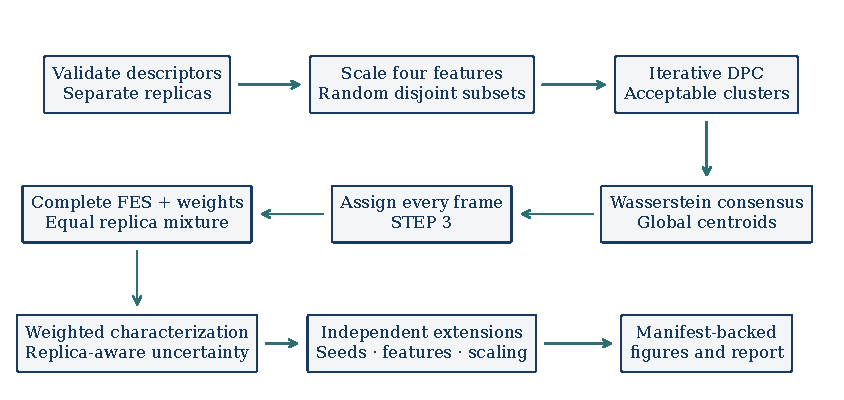
\includegraphics[width=\textwidth]{fig01_workflow.pdf}
\caption{Implemented analysis design. The primary branch separates geometric cluster discovery from statistical reweighting. Robustness experiments rerun designated stages independently. The FES grid has been validated, while empirical weighting remains blocked by energy-unit and construction provenance; this workflow diagram documents implementation, not successful completion of every box.}
\label{fig:workflow}
\end{figure}

Distances are computed in bounded blocks into a float32 matrix. Cutoff density is evaluated row by row without an additional floating kernel matrix. Silhouettes reuse that distance matrix, subject to the validity condition that the number of labels lies between two and $N-1$ \autocite{sklearnsilhouette}. The algorithm still has quadratic storage and potentially substantial repeated silhouette cost; the changes reduce avoidable allocations rather than changing its asymptotic scaling.

\section{STEP 2: Wasserstein consensus}
Only acceptable local clusters enter consensus. For clusters $A$ and $B$, the implemented source metric is
\begin{equation}
D(A,B)=\left[\sum_{f=1}^{4}W_1(A_f,B_f)^2\right]^{1/2}.
\label{eq:wasserstein}
\end{equation}
Here $W_1$ is the one-dimensional first Wasserstein distance between empirical marginal descriptor distributions \autocite{scipywasserstein}. Equation~\ref{eq:wasserstein} does not describe joint four-dimensional optimal transport. It can miss changes in dependence structure that leave every marginal distribution unchanged.

The reproduction configuration uses raw descriptors, matching the supplied code. This mixes descriptor scales and units in the aggregate norm; the paper does not fully resolve that scaling choice. The normalized alternative is retained as an explicit extension. Average-linkage agglomeration is followed by the source's cubic-spline elbow heuristic: smoothing parameter 5, with the maximum second derivative sought in the first 90\% of merge steps. Fewer than five local clusters or an entirely flat merge-height curve yields an explicit failure instead of an invented cut.

\section{STEP 3: final frame assignment}
Each global centroid is the mean normalized feature vector of all accepted local-cluster members assigned to that family. All analysis-window frames, including residuals and frames outside reduced discovery groups, are assigned once to the nearest centroid. Distance ties use deterministic label ordering. Centroids are not iteratively refitted after reassignment: doing so would introduce a k-means refinement absent from the documented baseline.

The final labels are stored with the original frame identities. This lets descriptor statistics, stability comparisons and any later structural mapping refer to exactly the same observations. Their molecular interpretation remains limited by the chosen descriptor representation.

\section{FES validation and interpolation}
The FES parser requires explicit axis names, extrema, grid counts, and nonperiodic status. It verifies row count, finite values including supplied derivative columns, coordinate spacing, unique Cartesian pairs, and agreement with the header. Row order is not assumed. A partial-download extension is rejected before parsing.

Interpolation uses SciPy's linear rectilinear-grid interpolator with bounds checking enabled \autocite{scipygrid,virtanen2020}. Every query must fall inside both axes. A bilinear analytic surface containing a mixed $\alpha\beta$ term provides an exact test, including boundary queries and shuffled rows. Missing cells and out-of-bounds queries are errors; no extrapolation or clipping is permitted.

\section{Statistical weights}
Equation~\ref{eq:finalweights} is evaluated in log space. Within replica $r$, normalized weights are
\begin{equation}
\widetilde w_{ri}=\exp\!\left[\ell_{ri}-\operatorname{logsumexp}_j(\ell_{rj})\right],
\qquad W_{ri}=\frac{\widetilde w_{ri}}{3}.
\label{eq:replicaweights}
\end{equation}
Equation~\ref{eq:replicaweights} gives each replica equal total mass, independently of the arbitrary log-weight offset or differences in raw weight sums. The recorded raw exponential is diagnostic only. If it is not representable, the output includes an explicit overflow/underflow status; normalized calculations remain based on log weights.

The intended frame table contains replica, source row, file line, frame index, time, physical CVs, interpolated free energy, raw log weight, raw weight/status, within-replica weight, pooled weight, and final label. No such real weighted table is reported in this release because FES energy-unit and construction provenance remain unverified.

\section{Weighted cluster characterization}
For a cluster, summing the pooled weights gives its relevance. Restricting those weights to its members gives the conditional descriptor mean and width. The width is the square root of the weighted central second moment: it describes heterogeneity within the family. Replica SEM addresses a different question, the variation of the relevance estimate across replicas, and is calculated from the separate replica populations.

The uncertainty extension keeps the fitted labels and supplied FES fixed while resampling contiguous observation blocks independently within each replica. It renormalizes the selected weights and recalculates populations for each draw. The resulting intervals would be conditional on that partition and FES; they do not incorporate uncertainty from reconstructing the FES, selecting a model or changing the clustering seed. This scope is recorded with the output.

\section{Software environment and reproducibility}
The modular implementation uses NumPy, SciPy, pandas, Matplotlib and scikit-learn; the key numerical and machine-learning libraries have established primary descriptions \autocite{harris2020,virtanen2020,pedregosa2011}. A locked environment records installed versions separately from published simulation versions. Snakemake expresses stage dependencies, while CLI commands provide the same functionality without notebooks \autocite{snakemakedocs,wratten2021}.

Each run begins with a manifest and resolved parameters. A supervisor records the worker's status and samples process-tree memory every 0.1 s, enforcing configured runtime and memory limits. Successful, failed, and blocked runs have distinct final statuses. Figures may be rebuilt only from a successful manifest after its output hashes are checked. The resulting record links each figure to the calculation and data that produced it.

\chapter{Reproduction and scientific code audit}
\section{Original implementation}
The supplied implementation puts input reading, replica separation, plotting, clustering and summary calculations in one script. Parsing the source identifies an Italian sentence without a comment marker at line 437, causing a syntax error before the analysis can run. The original is preserved exactly, including this defect, so that the audit can be checked against the supplied file.

The audit traces each calculation from its input to the quantity it would report. Reading the source shows what the script attempts to do, but no original execution manifest or complete numerical output set was located. Where the code differs from the paper, the method map records both versions and explains the correction made in the modular implementation.

\section{Identified methodological issues}
The original parser silently takes the first three segments separated by time resets and skips certain malformed lines. The new parser checks both the segment count and each row. Original group generation depends on a fixed list of 17 seeds, which would run out with smaller groups. The replacement uses local RNG streams and preserves every frame's identity. It makes the sampling reproducible but changes the exact subsets, so it is not claimed to reproduce the legacy script bit for bit.

The handling of residual frames changes which observations define a family. In the supplied code, rejected frames receive a generic label and every label enters consensus. Frames that failed the acceptance criteria can therefore influence the global centers. The modular version uses only accepted local clusters to discover families, then assigns the residual frames in STEP 3. Residuals still contribute to the final population without being treated as an accepted local cluster.

The original FES reader ignores the header information needed to check completeness and permits missing grid values with a warning. The weight function uses the nearest grid point and selects a boundary value for out-of-range queries. These choices can produce plausible-looking weights from invalid inputs. The replacement rejects incomplete grids and uses bilinear interpolation only within the grid bounds. The original partial download ended inside a numerical row and was rejected. The complete replacement received on 7 October passed grid validation; the earlier partial file remains unusable.

The original analysis weights cluster relevance but uses ordinary arithmetic means and standard deviations for the structural descriptors. Those summaries describe a different distribution from the weighted one specified in the paper's figure captions. The revised routines use the same weights for relevance and descriptor summaries within each cluster, and normalize replicas separately before pooling. Distribution width, replica SEM and bootstrap intervals remain separate quantities.

\begin{auditnote}
Correcting a calculation does not validate its input data or establish that the original simulation converged. The complete grid now passes validation, but its energy unit and construction procedure still need clarification before reweighting the real data.
\end{auditnote}

\section{Scientific V2 corrections: evidence unavailable}
The requested intermediate file \code{CLUSTERING40\_scientific\_v2.py} and its changelog were not located. The method map therefore marks that implementation as unavailable. None of the corrections in this report is attributed to the missing version. If supplied later, it should be checked by its hash, preserved unchanged, and compared with both the original and the modular implementation.

\section{Verification and numerical tests}
The current suite passed 36 tests, including strict parsing, interval boundaries, normalization, analytic bilinear interpolation, incomplete and duplicate grids, finite/bounds checks, weight sign, free-energy-offset invariance, equal replica masses, weighted moments, residual handling, final assignment, label-permutation agreement, and bootstrap separation of replicas. A seeded autoregressive fixture checks that the correlation estimator behaves plausibly for a known stationary process.

A complete synthetic test dataset exercises cluster discovery, consensus, all-frame assignment, final-bias weights, population tables, conditional bootstrap intervals and PDF generation. Its generated descriptors and analytic surface are used only for testing, not as Aβ40 observations. A further test checks repeatability by fitting the GMM extension to synthetic, separated observations. Tests with renamed labels and missing families check that the comparisons behave as intended. An archive-provenance test also checks that a source release cannot inherit the Git commit of an unrelated enclosing repository. These tests check numerical behavior; they cannot establish that a cluster represents a biological family.

\section{Remaining methodological ambiguities}
The main unresolved choices are the exact descriptor scaling in STEP 2, how the replica-averaged FES was constructed, and how the published cluster widths and uncertainties were defined. The supplied code also gives more detail than the paper about density ties and spline-based elbow selection. The repository identifies these choices as based on the supplied source; it does not imply that the paper fully specifies them.

These choices affect how the analysis is run and how its results can be compared. Raw Wasserstein scaling remains the reproduction setting; normalized scaling has a separate extension configuration. The complete numerical grid does not resolve how the FES was constructed. Any future difference in populations will need to be checked against these analysis choices before it is given a biological interpretation.

\chapter{RobustCluster-Aβ: robustness extension}
\section{Temporal correlation and effective sampling}
For each replica and baseline descriptor, the extension subtracts the mean and computes autocorrelation using an FFT-based convolution. Covariances use the common $1/N$ normalization. It pairs adjacent terms at positive lags and stops at the first pair whose sum is nonpositive. Each retained pair sum is then limited to the smallest pair sum seen so far. This gives the diagnostic
\begin{equation}
g=\max\!\left(1,1+2\sum_{k\in\mathcal K}\widehat\rho(k)\right),\qquad
N_{\mathrm{eff,corr}}=N/g,\qquad \tau_{\mathrm{int}}=g\Delta t/2.
\label{eq:correlation}
\end{equation}
In \cref{eq:correlation}, $\mathcal K$ denotes the lag contributions retained by this procedure; the implementation saves the lag at which summation stops. The convention includes the zero-lag half term in $\tau_{\mathrm{int}}$. Some definitions omit this term, so a reported ``correlation time'' needs an explicit convention.

Three checks help assess the estimate: whether a stopping lag was found, whether $N\geq50g$, and whether the absolute difference between first- and second-half means is at most 0.25 of the full-series standard deviation. The result is flagged if any check fails. These practical checks identify estimates with weak support from the available series; they are not a formal test that the process is stationary. More generally, an uncertainty estimate must be supported by the data and its sampling assumptions \autocite{grossfield2019,chodera2016}.

Weight concentration is assessed separately by
\begin{equation}
N_{\mathrm{eff,Kish}}=\frac{(\sum_i w_i)^2}{\sum_i w_i^2}.
\label{eq:kish}
\end{equation}
Equation~\ref{eq:kish} describes how unequal weights reduce the effective number of contributing observations, without correcting for dependence between them. It is not multiplied by, or automatically divided by, the correlation ESS. Combining the two effects would require a dependence calculation for the particular weighted observable and estimator. No Kish ESS is reported for the real data because their statistical weights have not been validated.

\section{Cluster stability across seeds}
Random grouping affects which local clusters are found, so the planned DPC seed experiment repeats discovery, consensus cutting and final assignment together. Simply renaming the labels of a fixed partition would not test this variation. The smoke profile uses two seeds, the separate pilot uses five, and the full profile, which has not been run, defaults to 20, with support for a 20--50-seed study.

Partitions are compared using the same source frames. ARI measures agreement regardless of the names assigned to clusters \autocite{hubert1985}. Families are then matched across runs to maximize their overlap, allowing Jaccard overlap, population variation and centroid movement to be summarized. Families without a match remain in the comparison, including those that appear or disappear. Considering only matched families could hide changes in cluster number even when those families look stable.

To compare centroids from different representations, the analysis uses the original four descriptors rescaled by the common baseline ranges. It therefore does not compare a PCA-space centroid directly with a raw-space centroid. Population variation across seeds measures sensitivity to the algorithm's random choices on the same ensemble. It differs from sampling uncertainty between independent replicas.

\section{Feature redundancy and PCA}
The completed lightweight diagnostics calculate the pooled Pearson correlation matrix and PCA after standardizing each baseline feature to zero mean and unit variance. The explained-variance spectrum shows how much of the variation in the observed descriptors lies along each principal component. It does not measure thermodynamic relevance or identify a slow physical mode.

The alternative clustering configurations retain all principal components, with optional whitening to scale each component to unit variance. Keeping all components makes PCA an orthogonal rotation of the standardized variables, preserving their Euclidean distances. Any difference from the min--max baseline would therefore come from standardization, whitening, numerical effects or a later analysis choice, not from discarding dimensions. This distinction matters when interpreting a future change in clustering.

\section{Independent GMM feature-ablation experiment}
The completed original experiment compares the four baseline descriptors with $\na$, $\nb$ and $R_g$ after removing SASA. It uses Gaussian mixtures in scalar descriptor space, a different model from both the published DPC pipeline and coordinate-based ShapeGMM. For a standardized observation $\mathbf{x}$,
\begin{equation}
p(\mathbf{x})=\sum_{j=1}^{K}\pi_j\mathcal{N}(\mathbf{x}\mid\symbf{\mu}_j,\symbf{\Sigma}_j),\qquad \sum_j\pi_j=1.
\label{eq:gmm}
\end{equation}
Equation~\ref{eq:gmm} approximates the sampled descriptor distribution. Its mixture coefficients are not equilibrium statistical weights. The implementation uses scikit-learn \autocite{pedregosa2011}; each component has a full covariance matrix, allowing the model to represent correlations between its features.

The experiment uses one fixed, replica-balanced fitting sample: 1,000 frames from each replica, selected with sampling seed 20261007. Feature means and standard deviations are fitted on those 3,000 rows and reused for the shared features in both representations. At each $K=2,\ldots,6$, five seeds (42--46) initialize separate models, each with a 500-iteration limit, tolerance $10^{-3}$ and covariance regularization $10^{-6}$. Using one initialization per fit exposes variation between local solutions instead of selecting the best of several starts. The protocol was committed before execution.

Every fitted model assigns a label to all 300,003 observations, including those used for fitting. ARI compares the four- and three-feature assignments at each seed and component count; the ten seed pairs are also compared within each representation. Matching clusters by maximum overlap shows which labels correspond across runs. The analysis records Jaccard overlap, unmatched families, and centroid shifts measured in the shared standardized three-feature space. It also records raw label fractions for each replica. These comparisons describe the same data used in the analysis; they do not test prediction on held-out data, and the ranges across runs are not confidence intervals.

Keeping the fitting subset fixed isolates the effects of feature representation and initialization. The experiment does not measure uncertainty from selecting that subset or remove temporal dependence. BIC is saved only for comparisons within a feature space; it is not compared across dimensions or used to identify a physical number of states. The planned DPC ablations remain separate experiments that require their own input and execution records.

\section{Wasserstein scaling sensitivity}
The raw consensus distance and the normalized alternative both combine separate distances for each descriptor; only the scaling changes. This tests the effect of one unresolved implementation choice. Raw SASA and radius-of-gyration values have different units and numerical ranges, so the variable with the larger range can have a disproportionate influence on the combined distance.

The normalized comparison would measure how scaling affects the result, but would not establish which implementation the original authors intended. Joint distances, sliced Wasserstein, energy distance and MMD could test other aspects of similarity between distributions in later studies. None replaces the current baseline.

\section{Reweighting sensitivity}
The optional comparison keeps the fitted partition fixed and compares the final-bias estimator with weights derived from verified \code{metad.rbias}. It examines the reweighted distributions of all four baseline descriptors and family relevance. With the labels unchanged, any differences can be traced to weighting rather than to changes in the partition.

The descriptor file contains a column named \code{metad.rbias}, but the original PLUMED configuration and evidence for its energy unit are missing. Input validation therefore blocks this optional comparison. The implementation keeps the estimators separate, as described in the primary literature and official PLUMED reference \autocite{tiwary2015,bonomi2009,plumedreweight}.

\section{Alternative density-based clustering}
DPA would provide a useful benchmark because it estimates density and identifies significant peaks differently \autocite{derrico2021}. The comparison should examine family number, location, population and correspondence using the same frames and validated weights. No DPA fit has been performed in this project.

Weighted ShapeGMM can analyze biased structural ensembles \autocite{sasmal2024}. Applying it here would require atomic structures, consistent atom selections and alignment, and a verified link between structures and descriptor rows. The structures cannot be recovered from scalar descriptors alone, so this comparison remains deferred.

\section{Optional external validation}
An Aβ40 ensemble constrained by experimental data could provide an independent comparison of global compaction and secondary-structure behavior \autocite{borthakur2025}. Before comparing values, the sequence, temperature, weights, atom selections and definitions of each observable must be checked. A mass-weighted $R_g$ and a Cα-only $R_g$, for example, need not have directly comparable distributions.

No external ensemble has been processed in this project. The assessment identifies the relevant study and the conditions needed for a valid comparison. Testing agreement with NMR/SAXS-constrained descriptors remains future work.

\chapter{Results}
\section{Available evidence and execution status}
The real descriptor table passes the implemented schema, finite-value, replica and interval checks. Each of the three segments contains \num{100001} rows at the source-labelled 20 ps spacing. Thus the data are suitable for the reported scalar-descriptor diagnostics, subject to the provenance assumptions described earlier. This validation does not independently establish simulation convergence or the correctness of upstream molecular definitions.

The reported diagnostics come from run \code{\DiagnosticRun}. Its recorded elapsed time is \DiagnosticSeconds{} s, and its sampled peak worker-process memory is \DiagnosticMemory{} MiB. These measurements describe this lightweight local run only. They are not estimates of full DPC runtime, nor evidence of HPC execution. The earlier reproduction attempt stopped at the missing-FES gate. Subsequent complete-grid validation and the independent GMM run have distinct manifests and do not convert that blocked attempt into a successful reproduction.

\begin{table}[htbp]
\centering
\begin{tabularx}{\textwidth}{@{}lX@{}}\toprule
Analysis & Evidence status\\\midrule
Input validation & Completed on the supplied Aβ40 descriptor table\\
Correlation matrix / PCA & Completed; unweighted biased-sample diagnostics\\
Autocorrelations / provisional ESS & Completed; every estimate flagged as unreliable\\
FES grid and interpolation & Completed; units/construction remain unverified\\
Weighted paper reproduction & Blocked: unit/construction provenance\\
GMM seed / SASA-ablation pilot & Completed; biased-sample geometric comparison\\
DPC seed / feature / scaling studies & Not completed; separate reproduction prerequisites\\
Time-dependent weight comparison & Blocked: FES and rbias unit/provenance requirements\\
Molecular representatives / ShapeGMM & Blocked: coordinate trajectory and mapping absent\\
External validation / Leonardo jobs & Not performed\\\bottomrule
\end{tabularx}
\caption{Scientific evidence available at release. Tests on synthetic fixtures are excluded from the empirical analysis statuses.}
\label{tab:status}
\end{table}

\section{Descriptor distributions and redundancy}
The pooled Rg--SASA Pearson correlation is \RgSasaCorrelation{}, whereas the correlation between the two secondary-structure descriptors is \AlphaBetaCorrelation{}. These are properties of the biased observation sample. The strong compaction/exposure correlation motivates a SASA-ablation experiment, but does not demonstrate that either variable is dispensable for every local family.

The first standardized principal component explains \PCAFirst{}\% of total variance, and the second explains \PCASecond{}\%, giving \PCATwo{}\% cumulatively. \Cref{fig:features} presents the numerical correlation matrix and spectrum. This concentration of variance supports examining redundant directions; it does not justify discarding a lower-variance variable without checking the effect on clustering and relevance.

\begin{figure}[htbp]
\centering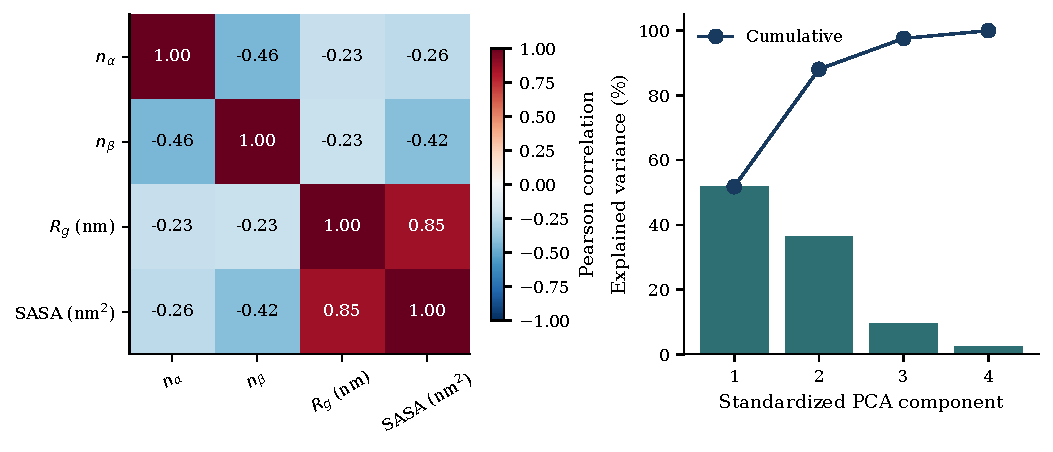
\includegraphics[width=\textwidth]{fig03_feature_diagnostics.pdf}
\caption{Computed diagnostics for the pooled, unweighted Aβ40 descriptor sample. Left: Pearson correlations of the four baseline descriptors. Right: explained variance of PCA after per-feature standardization, with cumulative variance shown by the line. These are geometric summaries of the biased sample and do not represent reweighted equilibrium probabilities.}
\label{fig:features}
\end{figure}

\Cref{fig:rawdistributions} shows per-replica empirical densities on common descriptor-specific bin edges. Each histogram is normalized by its own frame count and bin width. Differences between replicas are visible, but their equilibrium significance cannot be determined from these raw distributions alone. The plotted densities therefore describe the sampled trajectories, with no equilibrium correction.

\begin{figure}[htbp]
\centering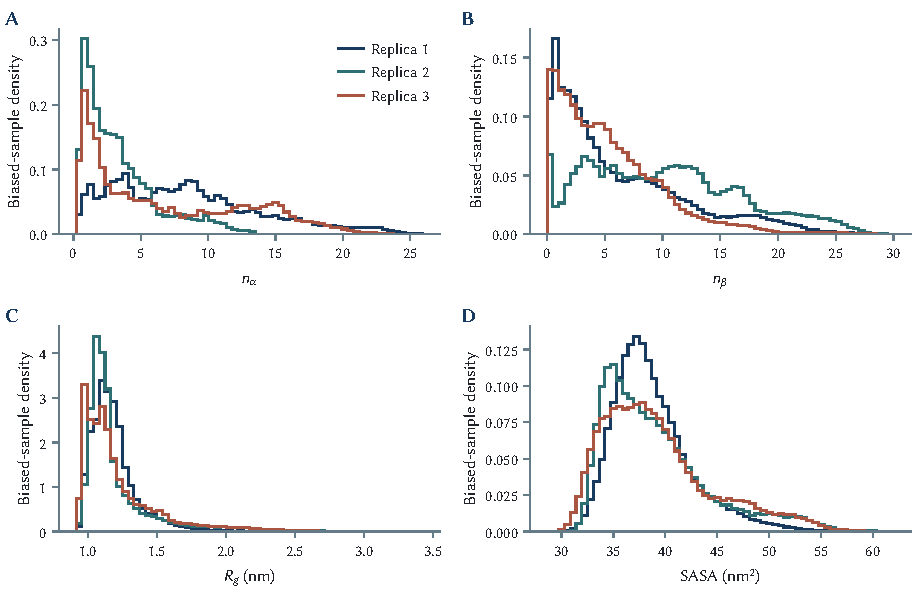
\includegraphics[width=.95\textwidth]{raw_descriptor_distributions.pdf}
\caption{Actual per-replica descriptor histograms over the supplied interval. Curves use common bin edges for each descriptor and independent density normalization. No final-bias or time-dependent statistical weights have been applied. Units follow the original script's labels and remain a recorded upstream-provenance assumption.}
\label{fig:rawdistributions}
\end{figure}

\section{Temporal correlation and provisional ESS}
The correlation diagnostics produce provisional ESS values ranging from \ESSMinimum{} to \ESSMaximum{} across the 12 replica--descriptor series, compared with \num{100001} raw frames in each series. All \UnreliableCount{} estimates fail at least one configured reliability heuristic. They should therefore be read as warning indicators of strong dependence and possible nonstationarity, not as precise counts of independent equilibrium conformations.

\Cref{tab:sampling} reports the estimator outputs together with the half-window mean shift. Several descriptors exhibit substantial differences between the first and second halves of the recorded interval. The extension does not convert those shifts into a formal rejection of the published convergence analysis, because the full bias history and corresponding convergence diagnostics are unavailable. It establishes that naive independent-frame uncertainty estimates would be poorly supported by the supplied stream.

\begin{table}[htbp]
\centering\small
\begin{tabular}{@{}clrrrr@{}}\toprule
Replica & Descriptor & $g$ & $\tau_{\mathrm{int}}$ (ns) & $N_{\mathrm{eff,corr}}$ & Half shift / SD\\\midrule
1 & $n_\alpha$ & 22067 & 220.7 & 4.5 & 1.28 \\
1 & $n_\beta$ & 11079 & 110.8 & 9.0 & 0.83 \\
1 & $R_g$ & 3679 & 36.8 & 27.2 & 0.27 \\
1 & SASA & 3490 & 34.9 & 28.7 & 0.36 \\
2 & $n_\alpha$ & 6259 & 62.6 & 16.0 & 0.37 \\
2 & $n_\beta$ & 10843 & 108.4 & 9.2 & 0.41 \\
2 & $R_g$ & 3951 & 39.5 & 25.3 & 0.33 \\
2 & SASA & 5325 & 53.2 & 18.8 & 0.17 \\
3 & $n_\alpha$ & 31742 & 317.4 & 3.2 & 1.61 \\
3 & $n_\beta$ & 5880 & 58.8 & 17.0 & 0.71 \\
3 & $R_g$ & 6259 & 62.6 & 16.0 & 0.88 \\
3 & SASA & 9958 & 99.6 & 10.0 & 0.87 \\
\bottomrule\end{tabular}

\caption{Computed correlation diagnostics. All entries are flagged as unreliable under the stated heuristics. The time scale is measured along the biased trajectory, using the source-labelled sampling interval. $g$ is statistical inefficiency; the final column is the absolute difference of half-window means divided by the full-series standard deviation. No physical relaxation-time interpretation is made.}
\label{tab:sampling}
\end{table}

\begin{figure}[htbp]
\centering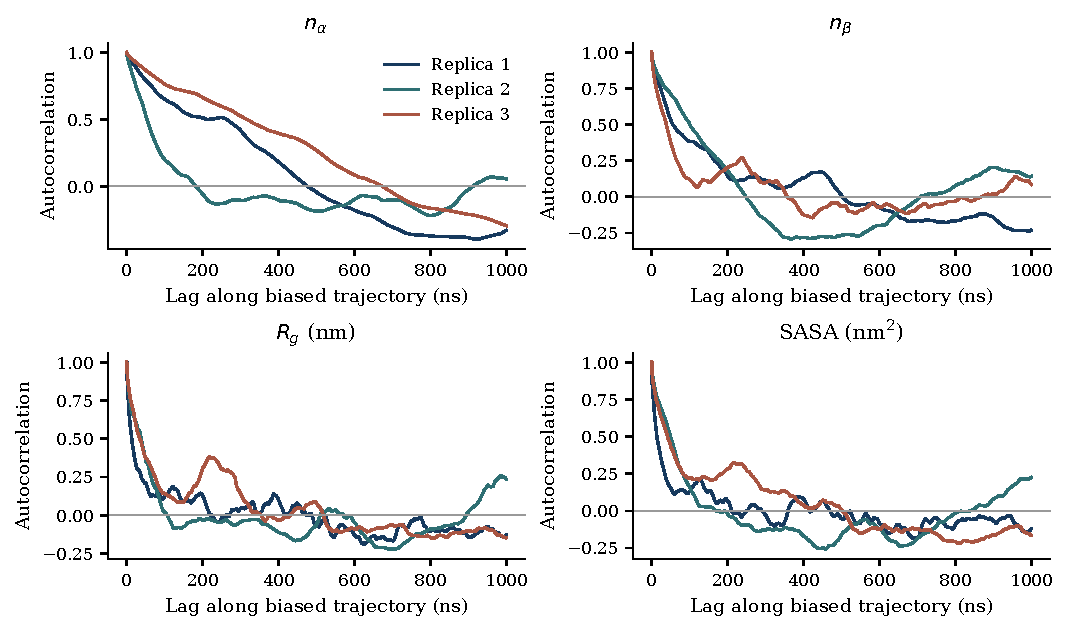
\includegraphics[width=.95\textwidth]{sampling_autocorrelations.pdf}
\caption{Autocorrelation functions computed separately for each replica and descriptor. The plotted curves cover the first half of the available lag window with a reduced plotting density; the estimator operates on the full, un-decimated ACF sequence. Long persistence and changing behavior across replicas reinforce the need for cautious uncertainty analysis. Lag is biased trajectory time, not recovered physical time.}
\label{fig:acf}
\end{figure}

\section{Complete FES validation}
The recovered file contains exactly 2,801 by 1,301 grid points: 3,644,101 rows with five finite columns, no duplicate coordinates and complete Cartesian coverage. Its nonperiodic axes span 0--28 and 0--13 at spacing 0.01. All 300,003 converted descriptor queries lie within those bounds, and bounded bilinear interpolation returns finite values for every query. The grid check is an input-integrity result; the energy column has no declared unit and is not assigned one solely because the source script assumes kJ/mol.

\section{Representation and initialization sensitivity}
The GMM pilot fitted \GMMModels{} models, all reporting convergence, in \GMMSeconds{} s with a sampled process-tree peak of \GMMMemory{} MiB. Convergence here means that the configured numerical stopping criterion was met, not that every model found the same or globally optimal solution. The comparison in \cref{fig:gmm} reveals substantial differences between component counts.
\begin{figure}[htbp]
\centering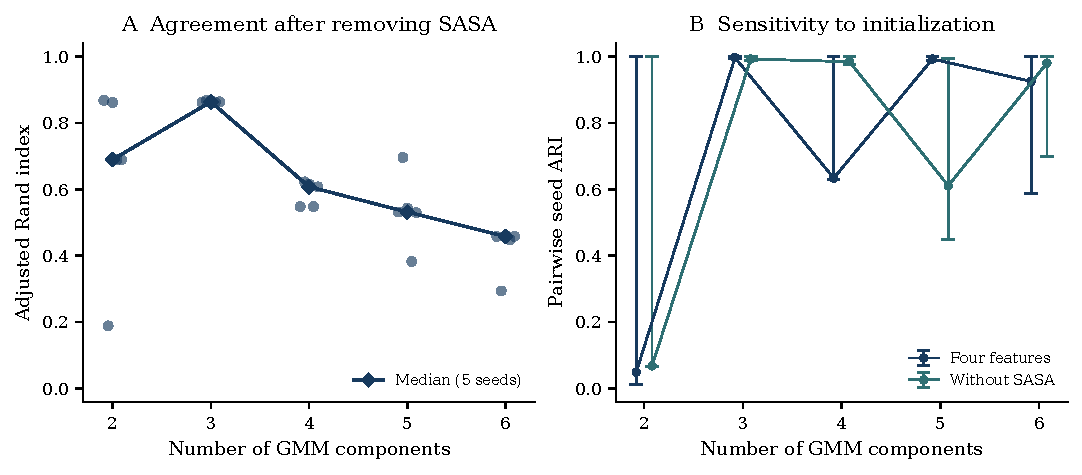
\includegraphics[width=\textwidth]{gmm_sensitivity.pdf}
\caption{Independent GMM sensitivity experiment on the biased descriptor sample. Left: four-feature versus SASA-ablated assignments at each of five seeds; diamonds mark medians. Right: within-space ARI over ten seed pairs; bars span observed minima and maxima, not confidence intervals. The fit subset is fixed across all models and evaluation includes fit rows.}
\label{fig:gmm}
\end{figure}
\begin{table}[htbp]\centering
\begin{tabular}{@{}crr@{}}\toprule Components & Median ablation ARI & Observed range\\\midrule
2 & 0.690 & 0.188--0.868 \\
3 & 0.864 & 0.862--0.868 \\
4 & 0.607 & 0.548--0.622 \\
5 & 0.531 & 0.382--0.696 \\
6 & 0.457 & 0.294--0.461 \\
\bottomrule\end{tabular}

\caption{Observed representation agreement across five paired initializations. Component count was varied by design; the table does not identify an optimal biological family count.}
\label{tab:gmm}
\end{table}
At three components, cross-representation ARI lies between 0.862 and 0.868, with approximately 95.3\% of frames retaining corresponding labels after maximum-overlap matching (median across seeds). Within-space seed agreement is also high: 0.994--1.000 with four descriptors and 0.988--1.000 without SASA. At two components, however, within-space ARI ranges down to 0.011 and 0.067, respectively. A single initialization would conceal this variability. The full matrices are retained in \cref{fig:seedmatrices}.

SASA removal preserves much of the three-component partition in this pilot, while agreement is lower or more variable at the other component counts. Thus the effect of removing SASA depends on the resolution and initialization of the fitted model. These comparisons concern assignments in the biased sample; weighted relevance and equilibrium populations have not been estimated.

\section{Analyses remaining unavailable}
Equilibrium cluster relevance, weighted family characterization and completed paper-DPC robustness remain unavailable. No molecular snapshots are created because the descriptor table has no atomic coordinates. The completed GMM experiment is an original descriptor-space extension, not a replacement for those stages.

\chapter{Discussion}
\section{A feature decision depends on the fitted model}
The completed experiment began with an apparently simple reason to reduce the feature set: radius of gyration and SASA are strongly correlated. The comparison shows why that observation alone is insufficient. Correlation summarizes a relationship over the whole sample, whereas clustering assigns individual observations using the geometry of all retained features. The assignments can change when a feature is removed even if that feature shares much of its variation with another one.

The three-component mixtures retained high agreement in this pilot, both across feature sets and across the tested initializations. The other component counts did not give the same pattern. This does not select three as the physical number of conformational states. It shows that the answer to the feature-removal question depends on how the data are represented by the chosen model. Keeping all tested component counts makes this dependence visible instead of reporting only the most stable case.

The fixed fitting sample helps isolate the comparison but also limits it. Both feature sets use the same observations and the same scaling for shared features. Differences are therefore not caused by selecting a new sample for each fit. However, the experiment says nothing directly about how those results would change with another fitting subset. Initializations and sample selection are different sources of uncertainty, and only the former was varied here.

\section{Connecting the extension to the published workflow}
The primary study uses density-peak discovery, consensus and reweighting to characterize conformational families \autocite{cadenelli2026}. The GMM pilot examines a narrower statistical question using the available descriptors. Its agreement scores neither reproduce the paper's family populations nor test the reported difference between Aβ40 and Aβ42. They also give no direct information about aggregation rates or toxicity.

A common difficulty links the two approaches: a numerical family still needs a physical interpretation. A stable Gaussian partition might summarize a broad descriptor distribution rather than separate metastable states. The consensus baseline likewise compares marginal descriptor distributions and can miss differences in their joint dependence. Structures, contacts and alternative representations would help examine these possibilities. An independently constrained ensemble could provide another comparison, provided the structures, weights and observable definitions are compatible \autocite{borthakur2025}.

\section{Sampling, weighting and the next comparison}
The temporal diagnostics limit the uncertainty claims available from the present data. Randomly drawing fitting frames does not remove correlation from the process that generated them. All replica--descriptor series fail at least one estimator check, so the small provisional ESS values should be treated as warnings rather than calibrated effective counts. Repeating fits across fitting subsets and time blocks would address sampling sensitivity more directly \autocite{grossfield2019}.

Weighting introduces a further issue. Grid completeness establishes that the FES can be queried, but not that its scale or construction is appropriate for the chosen estimator. Once those details are verified, unequal weights may concentrate the estimate on relatively few observations. That effect must be assessed separately from seed variation and temporal dependence. With only three replicas, uncertainty based on differences between replicas will also need cautious interpretation.

Saved labels, source tables and numerical tests allow the completed calculations to be checked. Equilibrium family populations remain dependent on the missing FES provenance. This boundary keeps further use of the project tied to its evidence \autocite{plumed2019,barker2022}.

\chapter{Internship outcomes and skills}
\section{Learning the molecular context}
The internship required more than applying a familiar statistical method to a new table. The assigned programme began with the concepts needed to interpret the data: amino acids, peptide bonds, protein structure and intrinsic disorder. Force fields, molecular dynamics and dihedral angles connected those concepts to simulation. The final task brought them together through examination of a clustering analysis and an independent investigation.

I used GROMACS, VMD and Python during the internship. Learning to use GROMACS was one of the more challenging parts of the internship for me. I found the process demanding at first, but I also enjoyed becoming more familiar with the software.

Saved configurations need not be independent observations, and their frequency in a biased simulation differs from their equilibrium probability. These points connect the molecular setting to statistics while showing why the origin of the data matters.

\section{Turning an observation into an analysis}
The Python project provides a concrete example. The descriptor analysis found a strong relationship between radius of gyration and SASA. Rather than treating this as a reason to remove SASA immediately, the independent experiment compared fitted assignments with and without it. The same fitting rows kept the comparison focused on the feature choice. Repeated initializations exposed variation that a single fit would have hidden.

Small programming decisions also became explicit parts of the analysis. Feature scaling is fitted on a specified sample and reused for later observations. A test checks that a large evaluation value cannot alter that transformation. Original frame identities are retained so that label arrays refer to the same observations. These details determine whether a difference comes from the method under investigation or an unintended change in preprocessing.

\begin{codepanel}{Fit once, reuse the same scale}{RobustCluster-Aβ / Python}
\lstinputlisting[style=editorialcode]{generated/fit_scaler.py}
\end{codepanel}


The modules, tests, configurations, source tables and plots document the work produced. Successful execution remains distinct from establishing the physical meaning of a cluster.

\section{My molecular-software interface projects}
I also created two personal software projects, \href{https://github.com/Alierkn/vmd-mcp}{VMD MCP} and \href{https://github.com/Alierkn/gromacs-mcp}{GROMACS MCP}. They use the Model Context Protocol to expose molecular-software operations through structured inputs and outputs. They are distinct from the Aβ40 descriptor analysis, but provide further examples of connecting scientific programs with Python interfaces.

\par\addvspace{8pt}\noindent
\begin{comparisonpanel}{VMD MCP: frame measurements}
The inspected source constructs Tcl commands for measurement and rendering. Its gyration function passes an atom selection and mass-weighting option to VMD, then returns frame-indexed values.
\end{comparisonpanel}\hfill
\begin{comparisonpanel}{GROMACS MCP: execution interface}
The inspected source includes preparation and analysis helpers. Its background-run interface checks paths and records output in a log.
\end{comparisonpanel}
\par\addvspace{8pt}
Contributor histories remain in the repositories. Appendix G links to the source versions inspected and pairs the code excerpts with genuine screenshots.

These interfaces organize requests; source code alone does not establish that a calculation ran. No reported Aβ40 trajectory is attributed to them. Comparing their outputs with the supplied descriptors would also require compatible selections and units: the inspected VMD gyration function documents angstroms, whereas the table is labelled in nanometres.

\section{What can be carried forward}
The report brings together the assigned learning programme, practical software use and calculations with saved outputs. Distinguishing them gives a clearer account than treating every planned task as completed. GROMACS and VMD use belongs to the practical experience; the descriptor diagnostics and GMM comparison belong to the recorded analysis.

The reusable outcome is a project whose steps can be examined. Each empirical figure has a source table, each calculation has settings, and each unavailable result has a reason. This organization can support further work once the FES units and construction are established. A Leonardo submission template is included for preparation, but no Leonardo job records exist. The reported computations remain local; further simulations or structural analyses will need their own execution records and validation.

\chapter{Conclusions and future work}
The internship materials support a study of how analysis choices affect the grouping of Aβ40 descriptors. Checking the supplied script against the published method identified problems in parsing, residual-cluster handling, FES interpolation, replica pooling and weighted summaries. The modular implementation makes the revised operations testable while preserving the original sources.

The independent GMM experiment gives the main completed comparison. Removing SASA largely preserves the tested three-component partition, but agreement changes at other component counts and with initialization. The Rg--SASA correlation therefore cannot decide the feature choice by itself. The experiment concerns one fitting subset and the biased descriptor sample; broader conclusions require further sampling comparisons and valid equilibrium weighting.

The next reproduction step is to establish the FES energy units and how the replicas were combined. A bounded real-data smoke run can then test the pipeline and measure resources before larger runs retain the published parameters. Seed, feature and Wasserstein-scaling experiments should compare the same frame identities so that changes in assignments have a clear meaning.

Additional inputs would enable distinct extensions. Verified bias-offset data would support time-dependent reweighting. Atomic trajectories with a reliable frame map would allow representative structures and coordinate-based analyses using tools such as MDAnalysis and ShapeGMM \autocite{michaud2011,sasmal2024}. An external ensemble comparison would require compatible observable definitions and appropriate data access.

The report's contribution is a documented analysis that can be inspected, with a completed test of feature sensitivity and explicit limits on what remains unknown. Its code and saved outputs provide a starting point for the remaining calculations. Equilibrium conformational families and their biological interpretation must follow from those calculations, rather than from the appearance of a stable partition alone.

\label{mainend}
\clearpage
\printbibliography
\appendix
\chapter{Full parameter table}
\label{app:parameters}
\section*{Iterative density-peak discovery}
Within each random group of about \num{30000} frames, discovery proceeds as follows.
\begin{protocolsteps}
\item \textbf{Generate candidates.} Start discovery at $d_c=1.3$, rank candidate centres by $\rho_i\delta_i$, and try 10 down to 2 centres.
\item \textbf{Check each cluster.} Require at least 300 members and a mean silhouette of at least 0.3 for acceptance.
\item \textbf{Choose the candidate.} Keep the one with the most acceptable clusters. A tie retains the earlier, higher-centre-count candidate.
\item \textbf{Continue on the remainder.} Remove accepted members and multiply $d_c$ by 0.9 before the next iteration.
\item \textbf{Stop discovery.} Stop below 300 remaining points or after five consecutive unsuccessful iterations. Residual frames receive their final labels only in STEP~3.
\end{protocolsteps}

\begingroup\small
\begin{longtable}{@{}>{\raggedright\arraybackslash}p{.34\textwidth}>{\raggedright\arraybackslash}p{.22\textwidth}>{\raggedright\arraybackslash}p{.36\textwidth}@{}}
\caption{Reproduction settings and execution profiles. These parameters are implemented but do not imply a completed empirical run.}\label{tab:parameters}\\
\toprule Parameter & Value & Evidence / role\\\midrule\endfirsthead
\multicolumn{3}{l}{\small\itshape Table \thetable\ continued}\\
\toprule Parameter & Value & Evidence / role\\\midrule\endhead
Replicas & 3 & Primary paper; observed table segmentation\\
Analysis interval & 1--3 μs & Published baseline; inclusive source-labelled ps boundaries\\
Temperature & 310 K & Published weighting parameter; no new MD run\\
Bias factor $\gamma$ & 10 & Published weighting parameter\\
Molar gas constant & 0.008314462618 kJ mol$^{-1}$ K$^{-1}$ & Implementation unit convention\\
CV conversions & $\alpha=\na/1.1$, $\beta=\nb/2.5$ & Published descriptor scaling\\
Baseline features & $\na$, $\nb$, $R_g$, SASA & Pooled min--max normalization\\
Initial $d_c$ & 1.3 & Published baseline\\
Cutoff multiplier & 0.9 & Published 10\% reduction\\
Center-count scan & 10 down to 2 & Published baseline\\
Minimum cluster size & 300 frames & Published acceptance criterion\\
Minimum mean silhouette & 0.3 & Published acceptance criterion\\
Failure stopping count & 5 & Consecutive iterations with no accepted cluster\\
Distance storage & float32 & Source-informed; blockwise construction\\
Consensus & Average linkage & Marginal Wasserstein norm\\
Elbow smoothing & $s=5$ & Supplied source heuristic\\
Elbow search range & First 90\% of merges & Supplied source heuristic\\
Final assignment & One nearest-centroid pass & No iterative refitting\\
Master seed & 42 & Default project configuration; recorded per run\\
Smoke / medium groups & 3,000 / 10,000 & Reduced execution profiles\\
Smoke / medium discovery groups & 2 / 3 & Not full-production evidence\\
Full group size & About 30,000 & All groups; full execution disabled\\
Seed counts & 2 smoke; 5 pilot/medium; 20 full default & Full robustness configurable; not performed\\
Bootstrap draws & 500 & Conditional moving-block extension; not performed on real weights\\
Resource policy & Bounded sequential local workers & Full execution held for review\\
\bottomrule
\end{longtable}
\endgroup
\addsec{Completed descriptor-only GMM pilot}
The protocol was committed before execution. Its four operations separate the choice of fitting observations from the comparisons made afterwards:
\begin{protocolsteps}
\item \textbf{Fix the sample.} Select 1,000 frames per replica with seed 20261007. Use the same 3,000 observations for every fit.
\item \textbf{Fit the transformation.} Estimate means and population standard deviations on those rows only. Share the transformation of retained descriptors between the four- and three-feature representations.
\item \textbf{Fit the models.} For each $K=2,\ldots,6$, use seeds 42--46: 50 fits overall. Each fit uses one initialization, at most 500 iterations, tolerance $10^{-3}$ and covariance regularization $10^{-6}$.
\item \textbf{Compare assignments.} Label all 300,003 frames, including fitting rows. Use five paired-seed ARIs to compare representations and ten seed pairs to compare initializations within each representation.
\end{protocolsteps}

The following settings belong to the successful independent experiment, not to the published DPC baseline. The fit sample and initializations were recorded before execution.
\begin{longtable}{@{}>{\raggedright\arraybackslash}p{.34\textwidth}>{\raggedright\arraybackslash}p{.22\textwidth}>{\raggedright\arraybackslash}p{.36\textwidth}@{}}
\caption{Settings of the completed GMM experiment, as recorded in its run manifest.}\label{tab:gmmparameters}\\
\toprule Parameter & Value & Evidence / role\\\midrule\endfirsthead
\multicolumn{3}{l}{\small\itshape Table \thetable\ continued}\\
\toprule Parameter & Value & Evidence / role\\\midrule\endhead
Fit sample & 1,000 per replica & 3,000 rows; shared across models\\
Sampling seed & 20261007 & Local NumPy generator\\
Feature spaces & Four descriptors; omit SASA & Same scaling for shared features\\
Scaling & Fit-sample mean and SD & No evaluation-data refit\\
Components & 2, 3, 4, 5, 6 & All counts retained in comparison\\
Initialization seeds & 42, 43, 44, 45, 46 & Paired across representations\\
Initializations per fit & 1 & 50 total fitted models\\
Covariance & Full & Regularization $10^{-6}$\\
Convergence settings & 500 iterations; tolerance $10^{-3}$ & All fits converged numerically\\
Evaluation & 300,003 rows & Includes fit rows; descriptive comparison\\
Resource limits & 600 s; 4 GiB & Sequential local worker\\
\bottomrule
\end{longtable}

\chapter{Mathematical derivations and estimator checks}
\label{app:derivations}
\section*{Gaussian hills and bias construction}
The accumulated potential can be written as a sum of local Gaussian hills:
\begin{equation}
V(s,t)=\sum_{t_k<t}h_k\exp\!\left[-\frac12\sum_a\frac{(s_a-s_a(t_k))^2}{\sigma_a^2}\right].
\label{eq:hills}
\end{equation}
In \cref{eq:hills}, $s$ is the CV vector, $t_k$ a deposition time, $h_k$ the hill height and $\sigma_a$ its width along coordinate $a$. Well-tempered heights follow $h_k=h_0\exp[-V(s(t_k),t_k)/(k_B\Delta T)]$ in molecular energy units; molar units require $R$ instead of $k_B$.

\section*{Why the sign of the final-bias correction is negative in FES form}
Under a static bias $V$, the observed configuration density is proportional to $\exp[-\beta_T(U+V)]$. Multiplying by $\exp(\beta_T V)$ recovers relative canonical density. The WT relation $V\simeq-(1-1/\gamma)F+C$ therefore gives the negative free-energy sign in \cref{eq:finalweights}. Applying $\exp(-\beta_T V)$ would reverse the correction. This derivation assumes that using a final bias is appropriate for the analyzed interval; it is not a proof that the supplied trajectories satisfy that assumption.

\section*{Kish effective sample size}
Unequal statistical weights require a separate diagnostic:
\begin{equation}
N_{\mathrm{eff,Kish}}=\frac{(\sum_i w_i)^2}{\sum_i w_i^2}.
\label{eq:kish}
\end{equation}
\Cref{eq:kish} measures weight concentration without correcting temporal dependence. It is not automatically combined with correlation ESS. No empirical Kish ESS is available without validated weights.

\section*{Equal-replica mixture and cluster moments}
Let $\widetilde w_{ri}$ sum to one within replica $r$. The pooled expectation of $A$ is $(1/3)\sum_r\sum_i\widetilde w_{ri}A_{ri}$. Cluster relevance uses $A$ equal to a membership indicator. For a conditional cluster mean, divide the pooled weighted sum of the descriptor by the pooled membership mass. Computing three conditional means and averaging them equally instead would answer a different question when cluster populations differ across replicas.

\section*{Bilinear interpolation test}
For a cell with fractional coordinates $u,v\in[0,1]$, interpolation combines its four corner values with weights $(1-u)(1-v)$, $u(1-v)$, $(1-u)v$, and $uv$. Their sum is one. Any surface $a+b\alpha+c\beta+d\alpha\beta$ is reproduced exactly within floating-point tolerance. The test suite includes such a mixed-term surface, reordered input rows, boundaries and invalid-grid cases, providing stronger evidence than checking a single grid node.

\chapter{Additional diagnostics and interpretation}
\label{app:diagnostics}
\begin{figure}[!htbp]
\centering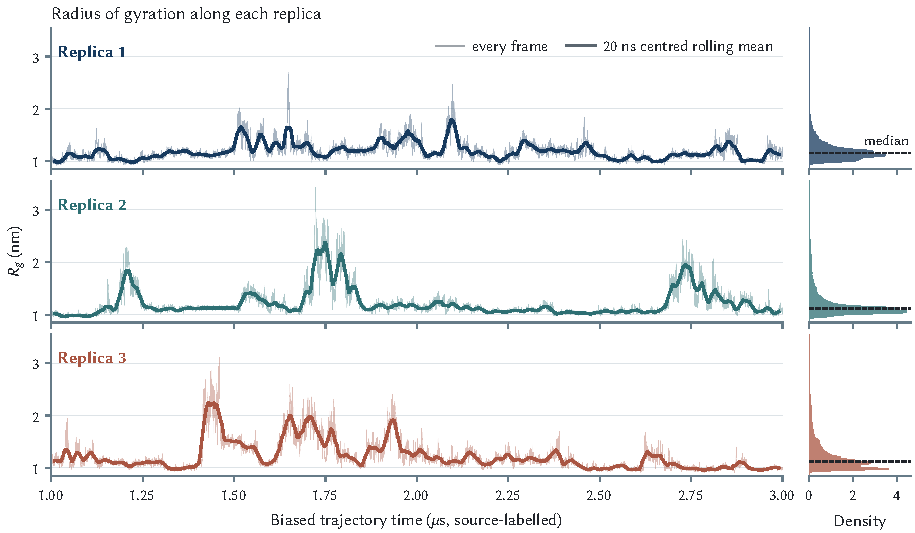
\includegraphics[width=\textwidth]{rg_timeseries.pdf}
\caption{Radius of gyration along the biased trajectory of each replica. Thin lines show every frame and bold lines a centred 20 ns (1,000-frame) rolling mean. The right-hand histograms are unweighted densities with dashed lines at the medians (1.153, 1.118 and 1.126 nm).}
\label{fig:rgtrace}
\end{figure}
\begin{table}[htbp]
\centering
\begin{threeparttable}
\caption{Agreement between feature sets across the five paired initializations.}
\label{tab:gmm}
\begin{tabular}{@{}crr@{}}\toprule Components & Median ablation ARI & Observed range\\\midrule
2 & 0.690 & 0.188--0.868 \\
3 & 0.864 & 0.862--0.868 \\
4 & 0.607 & 0.548--0.622 \\
5 & 0.531 & 0.382--0.696 \\
6 & 0.457 & 0.294--0.461 \\
\bottomrule\end{tabular}

\begin{tablenotes}[flushleft]\footnotesize
\item Component counts were specified for comparison, not selected as physical numbers of states.
\end{tablenotes}
\end{threeparttable}
\end{table}
\begin{figure}[!htbp]
\centering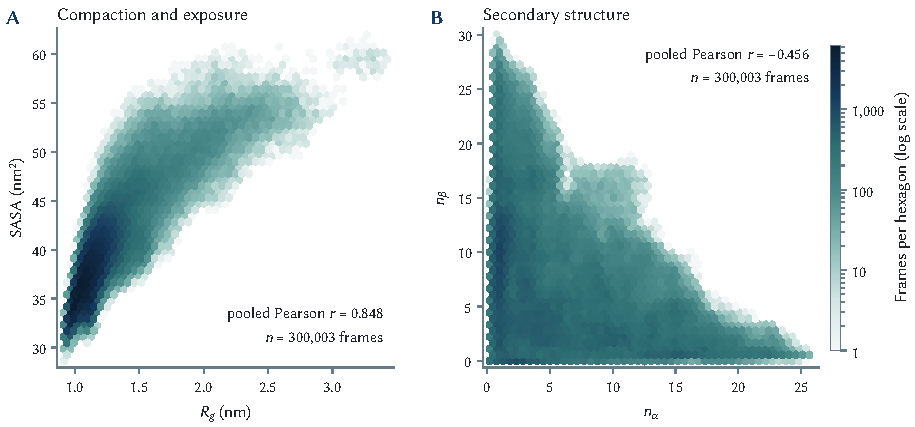
\includegraphics[width=\textwidth]{descriptor_landscape.pdf}
\caption{Unweighted descriptor landscape of the pooled sample (300,003 frames, three replicas, 1--3 μs). (A) Radius of gyration against SASA. (B) $\na$ against $\nb$. Shading is the log number of frames per hexagonal cell on a shared scale.}
\label{fig:landscape}
\end{figure}
\begin{figure}[!htbp]
\centering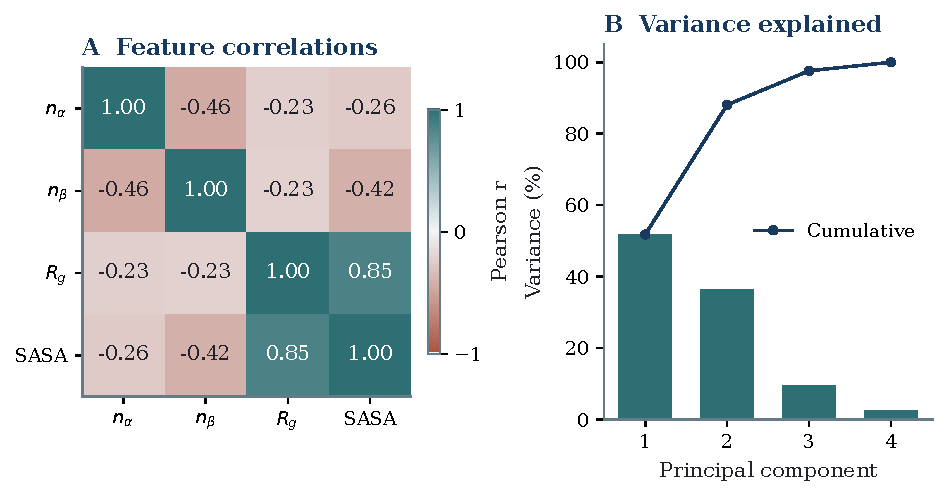
\includegraphics[width=\textwidth]{rebuild_features.pdf}
\caption{Relationships between the four descriptors in the pooled, unweighted sample. Left: Pearson correlation matrix. Right: variance explained by standardized PCA, with cumulative variance shown by the line.}
\label{fig:features}
\end{figure}
\begin{figure}[!htbp]
\centering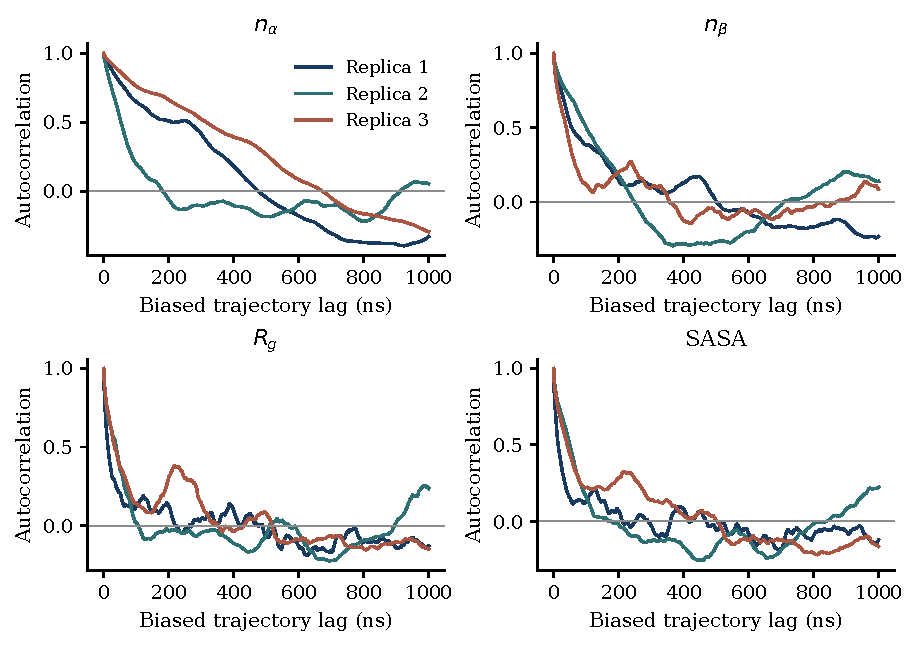
\includegraphics[width=.95\textwidth]{rebuild_autocorrelations.pdf}
\caption{Autocorrelation functions calculated separately for each replica and descriptor. For readability the figure displays a subset of lag points over the first half of the available window; estimation uses the full ACF sequence. The horizontal axis is biased trajectory time.}
\label{fig:acf}
\end{figure}

\begin{figure}[htbp]
\centering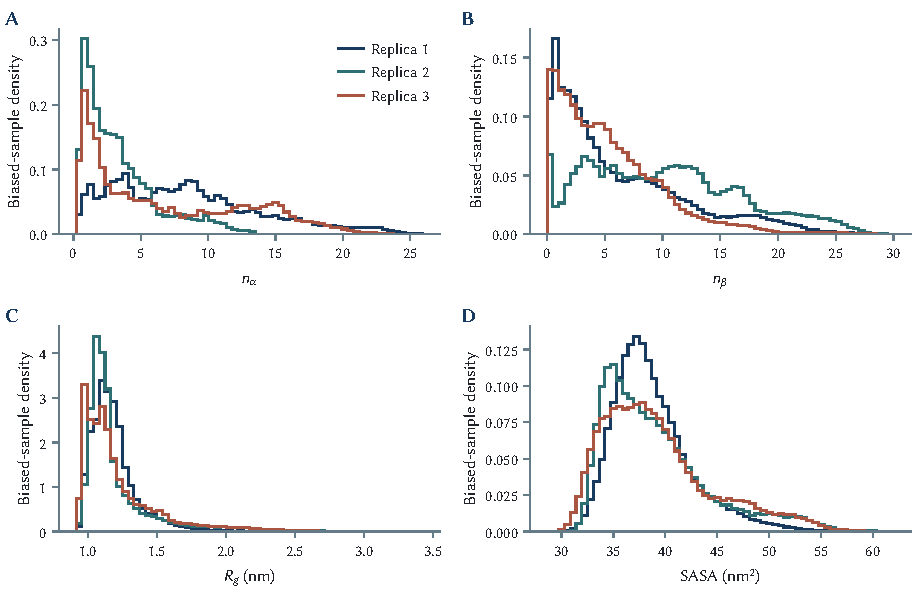
\includegraphics[width=\textwidth]{raw_descriptor_distributions.pdf}
\caption{Per-replica distributions of the recorded descriptors. Each descriptor uses common bin edges, with separate density normalization for each replica. The curves retain the simulation bias and are not equilibrium distributions. Units follow the source labels.}
\label{fig:rawdistributions}
\end{figure}
\begin{table}[htbp]
\centering
\caption{All recorded correlation estimates, each flagged as unreliable by at least one stated check. $g$ denotes statistical inefficiency. The half-window shift is the absolute difference of means divided by the full-series standard deviation. The time axis belongs to the biased trajectory.}
\label{tab:sampling}\small
\begin{tabular}{@{}clrrrr@{}}\toprule
Replica & Descriptor & $g$ & $\tau_{\mathrm{int}}$ (ns) & $N_{\mathrm{eff,corr}}$ & Half shift / SD\\\midrule
1 & $n_\alpha$ & 22067 & 220.7 & 4.5 & 1.28 \\
1 & $n_\beta$ & 11079 & 110.8 & 9.0 & 0.83 \\
1 & $R_g$ & 3679 & 36.8 & 27.2 & 0.27 \\
1 & SASA & 3490 & 34.9 & 28.7 & 0.36 \\
2 & $n_\alpha$ & 6259 & 62.6 & 16.0 & 0.37 \\
2 & $n_\beta$ & 10843 & 108.4 & 9.2 & 0.41 \\
2 & $R_g$ & 3951 & 39.5 & 25.3 & 0.33 \\
2 & SASA & 5325 & 53.2 & 18.8 & 0.17 \\
3 & $n_\alpha$ & 31742 & 317.4 & 3.2 & 1.61 \\
3 & $n_\beta$ & 5880 & 58.8 & 17.0 & 0.71 \\
3 & $R_g$ & 6259 & 62.6 & 16.0 & 0.88 \\
3 & SASA & 9958 & 99.6 & 10.0 & 0.87 \\
\bottomrule\end{tabular}

\end{table}
The saved tables contain per-replica raw descriptor counts, means, standard deviations, extrema, common-bin histograms, the full four-feature correlation matrix, PCA transformation parameters and explained variance, and the reported correlation-estimator diagnostics. The ACF figure is a plotting subsample, not the series used to estimate $g$. No weights are present in these real-data diagnostic summaries.

The half-window mean-shift diagnostic is descriptive. A large shift can arise from slow fluctuations, nonstationarity, or changing occupation of sampled regions. Its threshold is an explicit project heuristic. A low shift alone would not establish convergence, and no threshold outcome can recover an unbiased time scale from WT-MetaD time. Future evaluation should preserve these distinctions when adding weighted estimates.

\begin{figure}[htbp]
\centering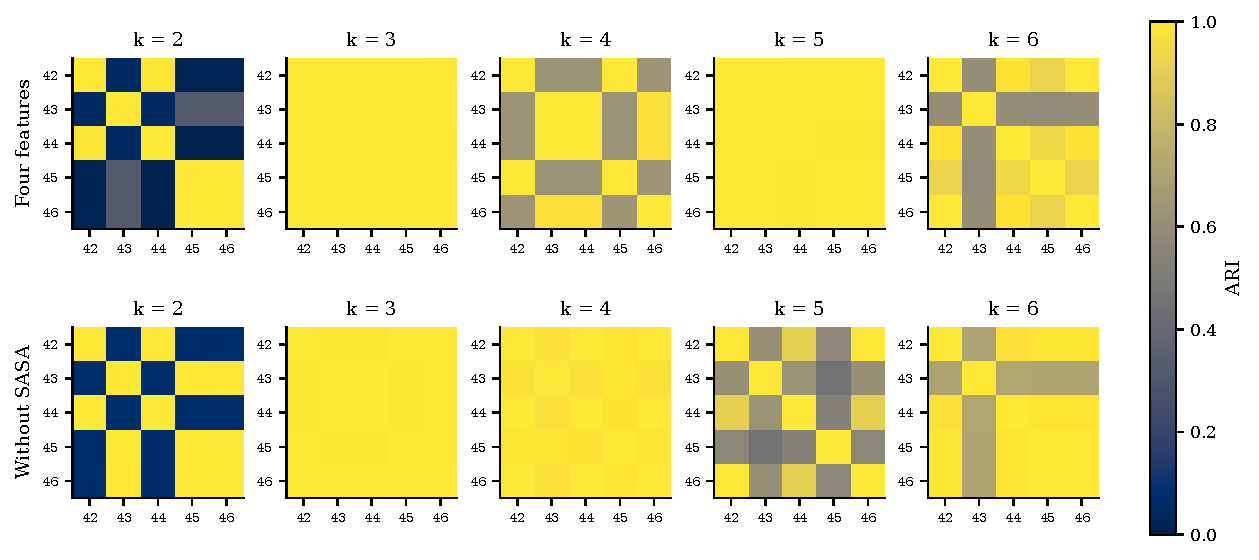
\includegraphics[width=\textwidth]{gmm_seed_matrices.pdf}
\caption{All pairwise seed ARIs from the GMM pilot. Columns show each tested component count; rows distinguish the four-feature and SASA-ablated representations. The diagonal is identity. All fits converged, so no entries are omitted. Similar numerical stopping status can coexist with different partitions.}
\label{fig:seedmatrices}
\end{figure}

\chapter{Code audit summary}
\label{app:codeaudit}
\begin{figure}[htbp]
\centering% Layered architecture of the robustcluster-abeta package (v0.3.0), drawn from the source tree:
% src/robustcluster_abeta/*.py imports, pyproject [project.scripts], config/*.yaml, workflows/Snakefile,
% scripts/, tests/ (36 tests passed in results/logs/*/pytest.log) and .github/workflows/ci.yml.
% gmm_ablation.py is called by cli.py directly (not by pipeline.py) and reads descriptors through io.py
% with its own scaler, so it receives no arrow from preprocessing.py.
% Solid frame: implemented and tested. Dashed frame: implemented; depends on the FES unit, run under the assumption stated in the report.
% Native TikZ; needs only arrows.meta (already loaded by preamble.tex).
\begin{tikzpicture}[
  font=\sffamily\footnotesize,
  every node/.append style={execute at begin node={\hyphenpenalty=10000\exhyphenpenalty=10000}},
  box/.style={draw=Navy!55,fill=CoolGrey,line width=.5pt,rounded corners=1.2pt,
    text width=#1,minimum height=10mm,align=center,inner sep=2.4pt,text=Ink,
    font=\sffamily\scriptsize},
  box/.default=27.2mm,
  pending/.style={box=#1,dashed,fill=white,draw=Navy!45},
  outbox/.style={box=#1,fill=Navy,draw=Navy,text=white},
  outbox/.default=27.2mm,
  frame/.style={draw=Teal!70,line width=.5pt,rounded corners=2pt,fill=Teal!6},
  flow/.style={-{Stealth[length=4.5pt,width=4pt]},draw=Navy!70,line width=.6pt},
  lane/.style={font=\sffamily\scriptsize\bfseries\addfontfeatures{LetterSpace=8},
    text=Teal,anchor=east},
  lanetop/.style={font=\sffamily\scriptsize\bfseries\addfontfeatures{LetterSpace=8},
    text=Teal,anchor=south}]
\def\ttl#1{{\footnotesize\bfseries #1}\\}
% main stack: columns centred at 15, 49, 83 mm (outer width 32 mm); right lane centred at 117 mm
% ---------------- INPUT
\node[box] (desc) at (15mm,0)  {\ttl{descriptor table}data/raw/\\{\fontsize{7.2}{8.6}\selectfont input\_clustering\_ab40.dat}};
\node[box] (fesin) at (49mm,0) {\ttl{FES grid}data/raw/\\FES\_AB\_40.dat};
\node[box] (yaml) at (83mm,0)  {\ttl{YAML config}config/*.yaml\\three run profiles};
% ---------------- I/O
\node[box] (io)  at (15mm,-15mm) {\ttl{io.py}read descriptors, check replicas};
\node[box] (fes) at (49mm,-15mm) {\ttl{fes.py}audit\_fes.py: grid structure, units};
\node[box] (man) at (83mm,-15mm) {\ttl{manifest.py}load config; hashes, run record};
\draw[flow] (desc) -- (io);  \draw[flow] (fesin) -- (fes);  \draw[flow] (yaml) -- (man);
% shared validation bar
\node[box=95.2mm,minimum height=5.5mm,fill=white,draw=Navy!40] (val) at (49mm,-25.5mm)
  {\textbf{validation.py} \textperiodcentered{} finite checks, time and memory budget, blocked vs failed states};
\draw[flow] (io) -- (io |- val.north);  \draw[flow] (fes) -- (fes |- val.north);
\draw[flow] (man) -- (man |- val.north);
% ---------------- SCALING
\node[box=95.2mm,minimum height=8mm] (pre) at (49mm,-35mm)
  {\ttl{preprocessing.py}min--max scaling of the four features \textperiodcentered{} random disjoint frame groups};
\draw[flow] (val) -- (pre);
% ---------------- ANALYSIS
\draw[frame] (0,-43mm) rectangle (72mm,-80mm);
\node[anchor=north west,inner sep=0pt,font=\sffamily\scriptsize,text=Teal] at (1.6mm,-44.3mm)
  {\textbf{pipeline.py} \textperiodcentered{} orchestrates the analysis stages};
\draw[flow] (36mm,-39mm) -- (36mm,-43mm);
\begin{scope}[every node/.append style={minimum height=12.5mm}]
  \node[box=19.4mm] (dpc)  at (12.3mm,-56mm) {\ttl{dpc.py}iterative density-peak clustering};
  \node[box=19.4mm] (con)  at (36mm,-56mm)   {\ttl{consensus.py}Wasserstein merge, frame assignment};
  \node[box=19.4mm] (stab) at (59.7mm,-56mm) {\ttl{stability.py}ARI, partition matching};
  \node[box=19.4mm] (stat) at (12.3mm,-71mm) {\ttl{statistics.py}ACF, Kish ESS, block bootstrap};
  \node[pending=43.1mm] (rw) at (47.85mm,-71mm) {\ttl{reweighting.py}FES-derived frame weights,\\equal-replica normalization};
  \node[box=22.4mm] (gmm) at (86.8mm,-71mm) {{\scriptsize\bfseries gmm\_ablation.py}\\Gaussian-mixture ablation, descriptor-only};
\end{scope}
\draw[flow] (dpc) -- (con);
% ---------------- OUTPUT
\node[box] (mf)  at (15mm,-92mm) {\ttl{results/manifests/}JSON run manifests};
\node[box] (tab) at (49mm,-92mm) {\ttl{results/tables/}CSV summaries};
\node[box] (fig) at (83mm,-92mm) {\ttl{plotting.py}figure scripts \textrightarrow{} results/figures/};
\draw[flow] (15mm,-80mm) -- (mf);
\draw[flow] (49mm,-80mm) -- (tab);
\draw[flow] (gmm.south) -- (gmm.south |- fig.north);
\draw[flow] (tab) -- (fig);
% ---------------- REPORT
\node[box] (prep) at (15mm,-107mm) {\ttl{prepare\_report.py}report/generated/*.tex};
\node[box] (bld)  at (49mm,-107mm) {\ttl{build\_report.py}latexmk \textperiodcentered{} LuaLaTeX};
\node[outbox] (pdf) at (83mm,-107mm) {\ttl{report.pdf}this report};
\draw[flow] (mf) -- (prep);
\draw[flow] (prep) -- (bld);  \draw[flow] (bld) -- (pdf);
\draw[flow] (fig.south) -- ++(0,-2.5mm) -| ([xshift=6mm]bld.north);
% ---------------- left lane labels
\foreach \y/\t in {0/INPUT,-15/{I/O},-25.5/CHECKS,-35/SCALING,-61.5/ANALYSIS,-92/OUTPUT,-107/REPORT}
  \node[lane] at (-2.5mm,\y mm) {\t};
% ---------------- right lane: entry points, tests and CI
\node[lanetop] at (117mm,-8mm) {ENTRY};
\node[box=23.2mm] (snk) at (117mm,-15mm) {\ttl{Snakefile}workflows/, via workflow\_stage.py};
\node[box=23.2mm,minimum height=12.5mm] (cli) at (117mm,-56mm) {\ttl{cli.py}console script robustcluster, seven commands};
\draw[flow] (snk) -- (cli);
\draw[flow] (cli) -- (72mm,-56mm);
\draw[flow] (cli.south) |- (gmm.east);
\node[lanetop] at (117mm,-85mm) {QUALITY};
\node[box=23.2mm] (tst) at (117mm,-92mm) {\ttl{tests/}38 pytest tests};
\node[box=23.2mm] (ci) at (117mm,-107mm) {\ttl{GitHub Actions}ruff + pytest, Python 3.12};
\draw[flow] (ci) -- (tst);
% ---------------- legend
\node[anchor=north,font=\sffamily\scriptsize,text=Ink] at (55mm,-115mm)
  {\tikz[baseline=-.6ex]\draw[Navy!55,fill=CoolGrey] (0,-1.2mm) rectangle (4.5mm,1.2mm);\enspace implemented and tested\qquad
   \tikz[baseline=-.6ex]\draw[Navy!45,dashed] (0,-1.2mm) rectangle (4.5mm,1.2mm);\enspace depends on the FES unit\qquad
   \tikz[baseline=-.6ex]\draw[Teal!70,fill=Teal!6] (0,-1.2mm) rectangle (4.5mm,1.2mm);\enspace called by pipeline.py};
\end{tikzpicture}

\caption{Architecture of the \code{robustcluster-abeta} package. Inputs pass through validation and scaling to the analysis modules orchestrated by \code{pipeline.py}; results go to manifest-backed tables and figures and then into this report. \code{gmm\_ablation.py} is the separate descriptor-only experiment of \cref{sec:task3}. The dashed module depends on the FES unit and was run under the assumption of \cref{sec:weighted}.}
\label{fig:architecture}
\end{figure}
\section*{Two numerical tests}
Two small examples from the 38-test suite show how a check can identify a numerical error without relying on the output of the full pipeline.

\paragraph{Interpolation with a known answer.}
An analytic bilinear surface includes a mixed-coordinate term, so a query between nodes tests both axes together. Reordering its rows must preserve the interpolated answer. Deleting or duplicating a grid point, or querying outside the bounds, must instead raise an error. The same fixture therefore checks both a valid calculation and the rejection of inputs for which that calculation would be inappropriate.

\paragraph{Normalization with an invariant.}
An arbitrary additive FES constant must disappear after weight normalization. A second check gives two replicas unequal numbers of frames and requires each to contribute half of the pooled mass. This catches pooling by row count, which would look correct on three equal-length replicas. Other weight tests check the formula's sign and weighted moments.

The remaining checks cover parsing, scaling, residual exclusion and final assignment. Renaming cluster labels must leave partition agreement unchanged; changing evaluation extremes must not alter a scaler fitted on fixed training rows. These checks isolate failures that could otherwise be mistaken for a change in the clustering method.

A synthetic end-to-end fixture exercises discovery, consensus, weighting, summaries and figure generation. Synthetic GMM cases check repeatability and missing-family handling. An autoregressive fixture probes the correlation estimator; an archive test prevents an unrelated enclosing Git repository from supplying false provenance. The fixtures establish software behaviour on known inputs (Scope~5).

The project inventory records immutable source hashes, table dimensions and missing inputs. The method map links each step to paper evidence, source behavior, the modular implementation and validation tests. The decision log records scientific category and expected effect. The open-questions register prevents uncertain provenance from being converted into hidden defaults.

Scientific V2 is absent, so the audit contains no invented intermediate diff. The supplied original remains excluded from execution and lint collection because its syntax error and top-level writes are part of the preserved evidence. New code is tested independently. Public source packaging excludes the raw table and original script until their redistribution rights are established.



The checked bibliography contains journal articles and official documentation records; its matrix links each citation to its question, method, relevance, and report section. Online-first dates and issue years are distinguished. References whose publisher verification remained unresolved are documented outside the BibTeX file rather than filled from memory.

\chapter{Reproducibility instructions and software environment}
\label{app:repro}
The project source, tests, configurations and this report are available at
\href{https://github.com/Alierkn/robustcluster-abeta}{RobustCluster-Aβ on GitHub}.
The \href{https://github.com/Alierkn/robustcluster-abeta/tree/main/src/robustcluster_abeta}{Python package}
and \href{https://github.com/Alierkn/robustcluster-abeta/tree/main/report}{LaTeX sources}
can be inspected separately or downloaded together using GitHub's \textit{Code / Download ZIP} option.
The repository guide distinguishes code verification and report regeneration from analyses requiring restricted inputs.

\begin{lstlisting}
python3.12 -m venv .venv
source .venv/bin/activate
python -m pip install -r requirements-lock.txt
python -m pip install --no-deps -e .
pytest -q
ruff check src tests scripts
robustcluster validate --config config/paper_reproduction.yaml
robustcluster diagnostics --config config/robustness.yaml
robustcluster cluster --config config/paper_reproduction_full.yaml --profile full
robustcluster reproduce --config config/paper_reproduction_full_assumed.yaml --profile full
\end{lstlisting}
The raw file must first be obtained and checked against its documented SHA256. The standalone commands and Snakemake workflow use the same package functions. The report imports successful diagnostics, FES-audit, GMM and figure manifests with matching hashes. Its generated editorial artwork and real browser screenshots have separate provenance records. LuaLaTeX, Biber and latexmk build the supplied report sources; current paths and tool versions are recorded in the build manifest.

The full-profile configurations record the measured resource estimates that justified enabling them (about 15 minutes and 4~GiB per clustering run). The configuration with the assumed FES unit states that assumption in its header and in every manifest it produces; once the unit is confirmed, only its two FES fields need to change. Outputs that would redistribute the FES or per-frame descriptor values stay local, with their hashes kept in the manifests. No calculation in this report used an HPC system \autocite{leonardodocs}.

\addsec{Software environment}
\begin{table}[htbp]
\centering
\begin{threeparttable}
\caption{Software versions for the reported local descriptor diagnostics.}
\label{tab:environment}
\begin{tabular}{@{}ll@{}}\toprule Component & Version in diagnostic manifest\\\midrule
Python & 3.12.6 \\
numpy & 2.5.3 \\
scipy & 1.18.1 \\
scikit-learn & 1.9.1 \\
pandas & 2.3.3 \\
matplotlib & 3.11.2 \\
robustcluster-abeta & 0.1.0 \\
\bottomrule\end{tabular}

\begin{tablenotes}[flushleft]\footnotesize
\item The GMM pilot manifest records the same versions. They do not describe the original authors' simulation environment. The complete dependency lock and report-tool versions are separate reproducibility artifacts.
\end{tablenotes}
\end{threeparttable}
\end{table}

\chapter{Personal projects and source-code evidence}\label{app:companion}
\begin{figure}[htbp]
\centering% Tooling map: where the student's tools sit relative to the analysis in this report.
% MCP projects labelled from the READMEs of github.com/Alierkn/vmd-mcp and github.com/Alierkn/gromacs-mcp.
% Dashed frame: personal project, not used to produce the supplied Abeta40 data.
% Native TikZ; needs only arrows.meta (already loaded by preamble.tex). Uses \abforty from preamble.tex.
\begin{tikzpicture}[
  font=\sffamily\footnotesize,
  every node/.append style={execute at begin node={\hyphenpenalty=10000\exhyphenpenalty=10000}},
  tool/.style={draw=Navy!55,fill=CoolGrey,line width=.5pt,rounded corners=1.2pt,
    text width=35mm,minimum height=14mm,align=center,inner sep=3pt,text=Ink,
    font=\sffamily\scriptsize},
  personal/.style={tool,dashed,fill=white,draw=Navy!45},
  outbox/.style={tool,fill=Navy,draw=Navy,text=white},
  flow/.style={-{Stealth[length=4.5pt,width=4pt]},draw=Navy!70,line width=.6pt},
  wraps/.style={flow,densely dashed,draw=Navy!45},
  lane/.style={font=\sffamily\scriptsize\bfseries\addfontfeatures{LetterSpace=8},
    text=Teal,anchor=east}]
\def\ttl#1{{\footnotesize\bfseries #1}\\}
% columns centred at 20.5, 63.5, 106.5 mm (outer width 41 mm, 2 mm gaps)
% ---------------- SIMULATION
\node[tool] (gmx) at (20.5mm,0)  {\ttl{GROMACS}molecular dynamics: topology, solvation, mdrun, trajectory analysis};
\node[tool] (vmd) at (63.5mm,0)  {\ttl{VMD}visualization and measurement: RMSD, R\textsubscript{g}, SASA, rendering};
% ---------------- PERSONAL MCP PROJECTS
\node[personal] (gmcp) at (20.5mm,-21mm) {\ttl{gromacs-mcp}MCP server: gmx pipeline, background mdrun};
\node[personal] (vmcp) at (63.5mm,-21mm) {\ttl{vmd-mcp}MCP server: headless VMD analysis, Tachyon rendering};
\draw[wraps] (gmcp) -- node[right,font=\sffamily\scriptsize,text=Navy!70,inner sep=1.5pt] {wraps} (gmx);
\draw[wraps] (vmcp) -- node[right,font=\sffamily\scriptsize,text=Navy!70,inner sep=1.5pt] {wraps} (vmd);
\node[anchor=west,text width=37mm,align=left,font=\sffamily\scriptsize\itshape,text=Audit,inner sep=0pt]
  at (88mm,-21mm) {personal Model Context Protocol projects: not used to produce the supplied \abforty{} data};
% ---------------- ANALYSIS
\node[tool] (data) at (20.5mm,-40mm) {\ttl{supplied \abforty{} data}descriptor table, FES grid};
\node[tool] (rc)   at (63.5mm,-40mm) {\ttl{robustcluster-abeta}analysis package of this report};
\node[tool] (py)   at (106.5mm,-40mm) {\ttl{Python stack}NumPy \textperiodcentered{} SciPy \textperiodcentered{} pandas\\scikit-learn \textperiodcentered{} Matplotlib};
\draw[flow] (data) -- (rc);
\draw[flow] (py) -- (rc);
% ---------------- REPORTING
\node[tool] (git) at (20.5mm,-60mm) {\ttl{Git / GitHub}version control, GitHub Actions CI};
\node[outbox] (tex) at (63.5mm,-60mm) {\ttl{LaTeX}LuaLaTeX report};
\draw[flow] (rc) -- (tex);
\draw[flow,draw=Navy!45] (git) -- (tex);
% ---------------- lane labels
\foreach \y/\t in {0/SIMULATION,-21/PERSONAL,-40/ANALYSIS,-60/REPORTING}
  \node[lane] at (-2.5mm,\y mm) {\t};
% ---------------- legend
\node[anchor=north east,font=\sffamily\scriptsize,text=Ink,align=left] at (127mm,-54mm)
  {\tikz[baseline=-.6ex]\draw[Navy!55,fill=CoolGrey] (0,-1.2mm) rectangle (4.5mm,1.2mm);\enspace tool or input\\[1pt]
   \tikz[baseline=-.6ex]\draw[Navy!45,dashed] (0,-1.2mm) rectangle (4.5mm,1.2mm);\enspace personal MCP project};
\end{tikzpicture}

\caption{Tools used during the internship. GROMACS and VMD belong to the simulation block; the Python stack, Git/GitHub and LaTeX produced the analysis and this report. Dashed boxes are personal Model Context Protocol servers, which were not used to produce the supplied Aβ40 data.}
\label{fig:tooling}
\end{figure}

\par\addvspace{8pt}\noindent
\begin{comparisonpanel}{VMD MCP: frame measurements}
The inspected source constructs Tcl commands for measurement and rendering. Its gyration function passes an atom selection and mass-weighting option to VMD, then returns frame-indexed values.
\end{comparisonpanel}\hfill
\begin{comparisonpanel}{GROMACS MCP: execution interface}
The inspected source includes preparation and analysis helpers. Its background-run interface checks paths and records output in a log.
\end{comparisonpanel}
\par\addvspace{8pt}

The following images are genuine browser captures from public, commit-specific GitHub source pages on 7 October 2026. They document implementation, not simulation execution. The full images are preserved unchanged; short accompanying searchable listings are a separate presentation format.
\begin{codepanel}{02\quad Measure each saved frame}{VMD MCP / source lines 250--266}
\lstinputlisting[style=editorialcode,firstnumber=250]{generated/vmd-mcp-excerpt.py}
\end{codepanel}
\begin{figure}[htbp]
\centering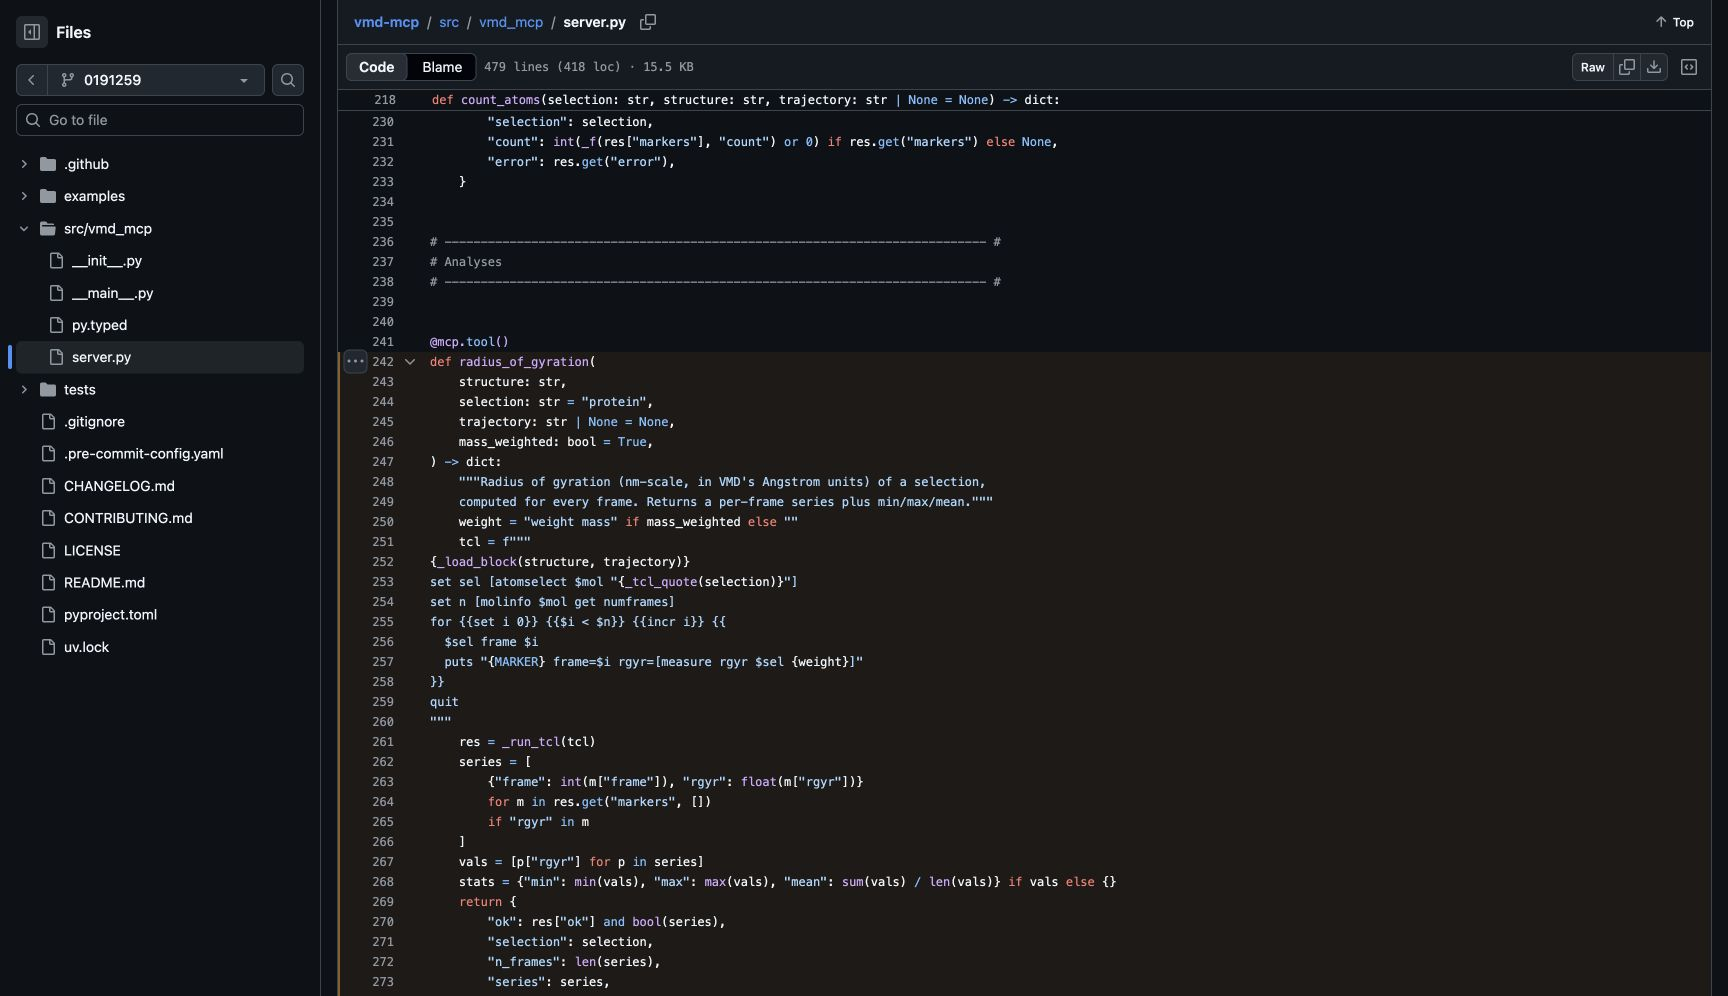
\includegraphics[width=.85\textwidth]{screenshots/vmd-gyration.jpg}
\caption{VMD MCP source at commit \texttt{0191259}: the gyration wrapper constructs a Tcl frame loop and parses marked values. The screenshot shows the repository tree, source path and real line numbers. The function's documented unit convention must be checked before comparison with other tools. \href{https://github.com/Alierkn/vmd-mcp/blob/01912595595bf0302124f57559e1e6a22095fb24/src/vmd_mcp/server.py\#L242-L278}{Open the inspected source}.}
\label{fig:vmdcode}
\end{figure}
\clearpage
\begin{codepanel}{03\quad Validate before starting a job}{GROMACS MCP / source lines 1452--1467}
\lstinputlisting[style=editorialcode,firstnumber=1452,gobble=8]{generated/gromacs-mcp-excerpt.py}
\end{codepanel}
\begin{figure}[htbp]
\centering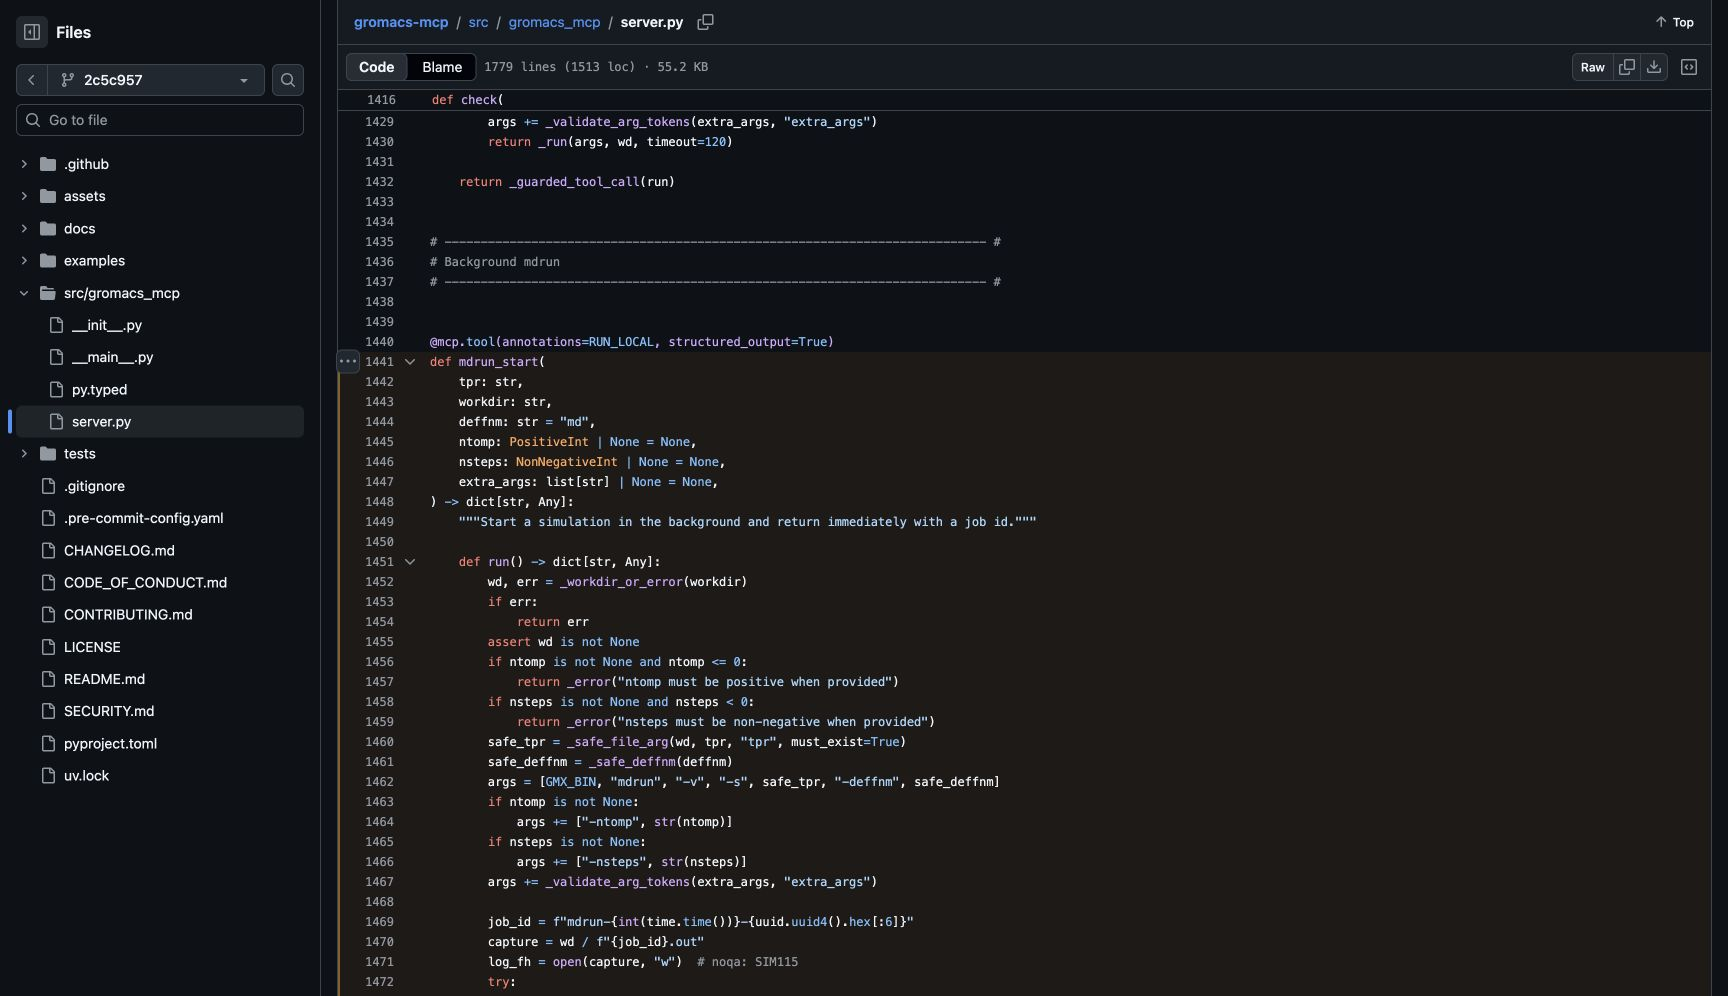
\includegraphics[width=.85\textwidth]{screenshots/gromacs-mdrun.jpg}
\caption{GROMACS MCP source at commit \texttt{2c5c957}: the background-run wrapper validates inputs, constructs the \texttt{mdrun} command and prepares an output log. This source view does not establish that an Aβ40 simulation was launched through the tool. \href{https://github.com/Alierkn/gromacs-mcp/blob/2c5c957c3f2c047888b63ae258ace3df34cb8773/src/gromacs_mcp/server.py\#L1441-L1479}{Open the inspected source}.}
\label{fig:gmxcode}
\end{figure}

\end{document}
